
\documentclass[11pt]{article}
\usepackage{amsmath,amsfonts,graphicx}
\usepackage{subcaption}  % For subfigures
\usepackage{float}       % For the [H] placement specifier
\usepackage{authblk}
\usepackage{geometry}
\geometry{margin=1in}
\usepackage{hyperref}
\usepackage{xcolor}

\title{Summary of Recent Research on Exact Quantum Many-Body Scars}
\author{Camilla Polvara}
\date{\today}

\begin{document}

\maketitle

\section*{Overview}

This document summarizes recent research focused on \textbf{exact quantum many-body scars} in spin systems, where analytic expressions for the scarred eigenstates are known. These studies circumvent the need to analyze the full Hamiltonian spectrum, instead targeting entanglement properties and reduced density matrices (RDMs) of analytically understood scarred states. All models are assumed to be in 1-dimension and to have periodic boundary conditions (PBC), unless otherwise specified.

\vspace{0.5cm}

\section*{1. Dimer State Scar}
\begin{itemize}
    \item \textbf{Model:} Spin-1/2 MG-like model featuring an exact dimer scar state.\\
    This is a one-dimensional spin-$\tfrac{1}{2}$ model with two- and three-body interactions. The Hamiltonian of the model depends on a parameter $t \in \mathbb{R}$ and is given by
    
    \begin{equation}
    H(t) = H_{\mathrm{MG}} + t\, C_{\mathrm{SC}},
    \end{equation}
    where
	\begin{equation}
	H_{\mathrm{MG}} = \sum_{j=1}^{L} \left[ \left( \mathbf{S}_j + \mathbf{S}_{j+1} + \mathbf{S}_{j+2} \right)^2 - \frac{3}{4} \right],
	\label{eq:HMG}
	\end{equation}
	\begin{equation}
	C_{\mathrm{SC}} = \sum_{j=1}^{L} \mathbf{S}_j \cdot \left( \mathbf{S}_{j+1} \times \mathbf{S}_{j+2} \right),
	\label{eq:CSC}
	\end{equation}
	and $\mathbf{S}_j = \left(S^x_j, S^y_j, S^z_j\right)$ is the spin-$\tfrac{1}{2}$ operator acting on site $j$:  
	\begin{align}
	S^x_j &= \frac{1}{2}
	\begin{pmatrix}
	0 & 1 \\
	1 & 0
	\end{pmatrix}_j, \\
	S^y_j &= \frac{1}{2}
	\begin{pmatrix}
	0 & -i \\
	i & \phantom{-}0
	\end{pmatrix}_j, \\
	S^z_j &= \frac{1}{2}
	\begin{pmatrix}
	1 & 0 \\
	0 & -1
	\end{pmatrix}_j.
	\end{align}
	
	The first term $H_{\text{MG}}$ is the Hamiltonian of the Majumdar-Ghosh model (which has the dimer states as ground states), while the second term $C_{\text{SC}}$ is the scalar spin chirality.\\ 
	

    
     There is just one scarred state, which is the ground state of the Majumdar-Ghosh Hamiltonian, and it's given by the singlet state:
    
    \begin{equation}
    | \text{dimer} \rangle = \left( 2 + \left( -\frac{1}{2} \right)^{\frac{L}{2} - 2} \right)^{-\frac{1}{2}} \left( |\Psi_1\rangle + |\Psi_2\rangle \right).
    \end{equation}

    where $L$ is the (even) number of sites, and
    
    \begin{align}
    &|\Psi_1\rangle = | \text{sing} \rangle_{1,2} \otimes | \text{sing} \rangle_{3,4} \otimes \cdots \otimes | \text{sing} \rangle_{L-1,L}, \\
    &|\Psi_2\rangle = | \text{sing} \rangle_{2,3} \otimes | \text{sing} \rangle_{4,5} \otimes \cdots \otimes | \text{sing} \rangle_{L,1},
    \end{align}
    
    are the two dimer states, with
    
    \begin{equation}
    | \text{sing} \rangle_{i,j} = \frac{1}{\sqrt{2}} \left( | \uparrow \downarrow \rangle_{i,j} - | \downarrow \uparrow \rangle_{i,j} \right).
    \end{equation}
    
    $| \text{sing} \rangle_{i,j}$ the normalized spin singlet between sites $i,j$.\\
    The scarred state is annihilated by $C_{\text{SC}}$ (as well as by $H_{\text{MG}}$), and thus it is a zero-energy eigenstate of $H$: $H(t)| \text{dimer} \rangle = 0$.
       
    \item \textbf{Reference:} \href{https://journals.aps.org/prb/abstract/10.1103/PhysRevB.108.155102}{Phys. Rev. B 108, 155102 (2023)}.
    \item \textbf{Analysis:}
    \begin{itemize}
        \item Verified the entanglement entropy against the analytic prediction from the paper.\\ For $L=14,16,18$:
        
        \begin{equation}
        S_A \approx 1.386 \approx 2 \ln 2
        \end{equation}
        
        Because $S_A$ evaluates to $\approx 2 \ln 2$ for increasing $L$, the dimer scar satisfy the \textit{Area Law} for entanglement: in one dimension, the entanglement entropy remains constant with increasing system size.
        
        \item Computed the ranks of all 2-site, 3-site, and 4-site adjacent reduced density matrices:
        
	\begin{table}[h]
	\centering
	\begin{tabular}{|c|ccc|}
	\hline
	\textbf{Dimer scar} & \multicolumn{3}{c|}{\textbf{RDM  Rank}} \\
	\cline{2-4}
	& \textbf{2-sites} & \textbf{3-sites} & \textbf{4-sites} \\
	\hline
	\text{$| \text{dimer} \rangle$} & 4 & 4 & 5 \\
	\hline
	\end{tabular}
	\caption{RDM ranks for 2, 3, and 4 adjacent sites in the dimer scar state for $L=18$.}
	\label{tab:ranks}
	\end{table}

\end{itemize}
\end{itemize}

\vspace{0.3cm}

\section*{2. Domain-Wall Conserving Spin-1/2 Model}
\begin{itemize}
    \item \textbf{Model:} Spin-1/2 model with domain-wall conserving dynamics.\\
    
     For a system $L$ spins-$\tfrac{1}{2}$ on a chain, the Hamiltonian reads
	\begin{equation}
	H = \sum_{i=1}^{L} \left[ \lambda \left( \sigma^x_i - \sigma^z_{i-1} \sigma^x_i \sigma^z_{i+1} \right) + \mu\, \sigma^z_i + J\, \sigma^z_i \sigma^z_{i+1} \right]
	\equiv H_\lambda + H_z + H_{zz},
	\label{eq:H}
	\end{equation}
    where $\sigma^{x,y,z}_i$ are Pauli matrices defined on site $i$.

	

    \item \textbf{Reference:} \href{https://journals.aps.org/prb/abstract/10.1103/PhysRevB.101.024306}{Phys. Rev. B 101, 024306 (2020)}.
    \item \textbf{Analysis:}
    \begin{itemize}
        \item Restricted study to analytically known scarred eigenstates.\\ There are two towers of scars, both of length $L/2$ for OBC and $L/2 + 1$ for PBC.\\
         The first tower is described by:
	 \begin{equation}
	|S_n\rangle = \frac{1}{n! \sqrt{\mathcal{N}(L, n)}} \left(Q^\dagger\right)^n |\Omega\rangle, \quad n = 0,\hdots,L/2 - 1 \, (L/2)
	\end{equation}
	
	where $|\Omega\rangle = |0 \cdots 0\rangle$ and, for PBC, $\mathcal{N}(L, n) = \frac{L}{n} \binom{L - n - 1}{n - 1}$ (\textcolor{red}{not defined for $n=0$, even though it describes the first scar of the tower, i.e. state $|\Omega\rangle $}). $Q^\dagger$ is 	the ladder operator, defined as:
	
	\begin{equation}
	Q^\dagger = \sum_{i = 1}^{L} (-1)^i P^0_{i-1} \, \sigma^+_i \, P^0_{i+1}, 
	\end{equation}
	
	where $\sigma_j^\pm = \frac{1}{2} (\sigma_j^x \pm i \sigma_j^y)$ and $P^0_i = \frac{1}{2} (1 - \sigma^z_i)$ is the local projector onto spin down.\\
        The second tower, related to the first one, is described as 
        \begin{equation}
	|S'_n\rangle = G |S_n\rangle = \frac{1}{n! \sqrt{\mathcal{N}(L, n)}} \left(Q'^\dagger\right)^n |\Omega'\rangle, \quad n = 0,\hdots,L/2 - 1 \, (L/2)
	\end{equation}
	
	\noindent where $G = \prod_{i=1}^L \sigma_i^x$ is a $\mathbb{Z}_2$ transformation that flips all spins, 
	$|\Omega'\rangle = |1 \cdots 1\rangle$, and
	
	\begin{equation}
	Q'^\dagger = G Q^\dagger G = \sum_{i = 1}^{L} (-1)^i P^1_{i-1} \, \sigma^-_i \, P^1_{i+1},
	\end{equation}
	
	\noindent with $P^1_i = \frac{1}{2}(1 + \sigma^z_i)$ the local projector onto spin up.\\
	Both scar towers are annihilated by $H_{\lambda}$, which breaks U(1): $H_{\lambda} |S_n\rangle = H_{\lambda} |S'_n\rangle = 0$.
        \item Computed entanglement entropy and verified its consistency with the original publication, where only $|S_4\rangle$ for L=18 sites was considered (with OBC!)
        
        \begin{equation}
        S^{\,|S_4\rangle}_A \approx 1.22 \approx \frac{1}{2} \ln \left(\frac{18 \pi}{8}\right) + \frac{1}{4}
        \end{equation}
        
        For generic $L$, $S^{\,|S_4\rangle}_A$ scales logarithmically with system size, i.e. $S^{\,|S_4\rangle}_A = \frac{1}{2} \ln \left(\frac{\pi L}{8}\right) + \frac{1}{4}$. Because $S^{\,|S_4\rangle}_A$ is at the top of the tower - it has maximum possible 				value of entanglement entropy among the scars - we can assume that all scars have sub-volume scaling with system size, i.e. constant or at most logarithmic.
        
        \item Ranks of adjacent 2-site, 3-site, and 4-site (adjacent) RDMs assessed, for both towers
        
        \begin{table}[H]
	\centering
	\begin{tabular}{|c|ccc|}
	\hline
	\textbf{$|S_n\rangle$} & \multicolumn{3}{c|}{\textbf{RDM Rank}} \\
	\cline{2-4}
	& \textbf{2-sites} & \textbf{3-sites} & \textbf{4-sites} \\
	\hline
	 n = 1 & 2 & 2 & 2 \\
	 n = 2 & 3 & 5 & 5 \\
	 n = 3 & 3 & 5 & 7 \\
	 n = 4 & 3 & 5 & 7 \\  
	 n = 5 & 3 & 5 & 7 \\
	 n = 6 & 3 & 5 & 7 \\
	 n = 7 & 3 & 5 & 7 \\
	 n = 8 & 3 & 5 & 6 \\
	\hline
	\end{tabular}
	\caption{RDM ranks for 2, 3, and 4 adjacent sites in the $|S_n\rangle$ scar tower for $L=18$.}
	\label{tab:ranks1}
	\end{table}

	 \begin{table}[H]
	\centering
	\begin{tabular}{|c|ccc|}
	\hline
	\textbf{$|S'_n\rangle$} & \multicolumn{3}{c|}{\textbf{RDM Rank}} \\
	\cline{2-4}
	& \textbf{2-sites} & \textbf{3-sites} & \textbf{4-sites} \\
	\hline
	 n = 1 & 2 & 2 & 2 \\
	 n = 2 & 3 & 5 & 5 \\
	 n = 3 & 3 & 5 & 7 \\
	 n = 4 & 3 & 5 & 7 \\  
	 n = 5 & 3 & 5 & 7 \\
	 n = 6 & 3 & 5 & 7 \\
	 n = 7 & 3 & 5 & 5 \\
	 n = 8 & 3 & 5 & 6 \\
	\hline
	\end{tabular}
	\caption{RDM ranks for 2, 3, and 4 adjacent sites in the $|S'_n\rangle$ scar tower for $L=18$.}
	\label{tab:ranks2}
	\end{table}
	
	The chain length $L$  dependence of the 2,3,4-sites RDM of the scar at the top of both tower was investigated too.
	
	\begin{figure}[H]
    \centering
    % First image
    \begin{subfigure}{0.45\textwidth}
        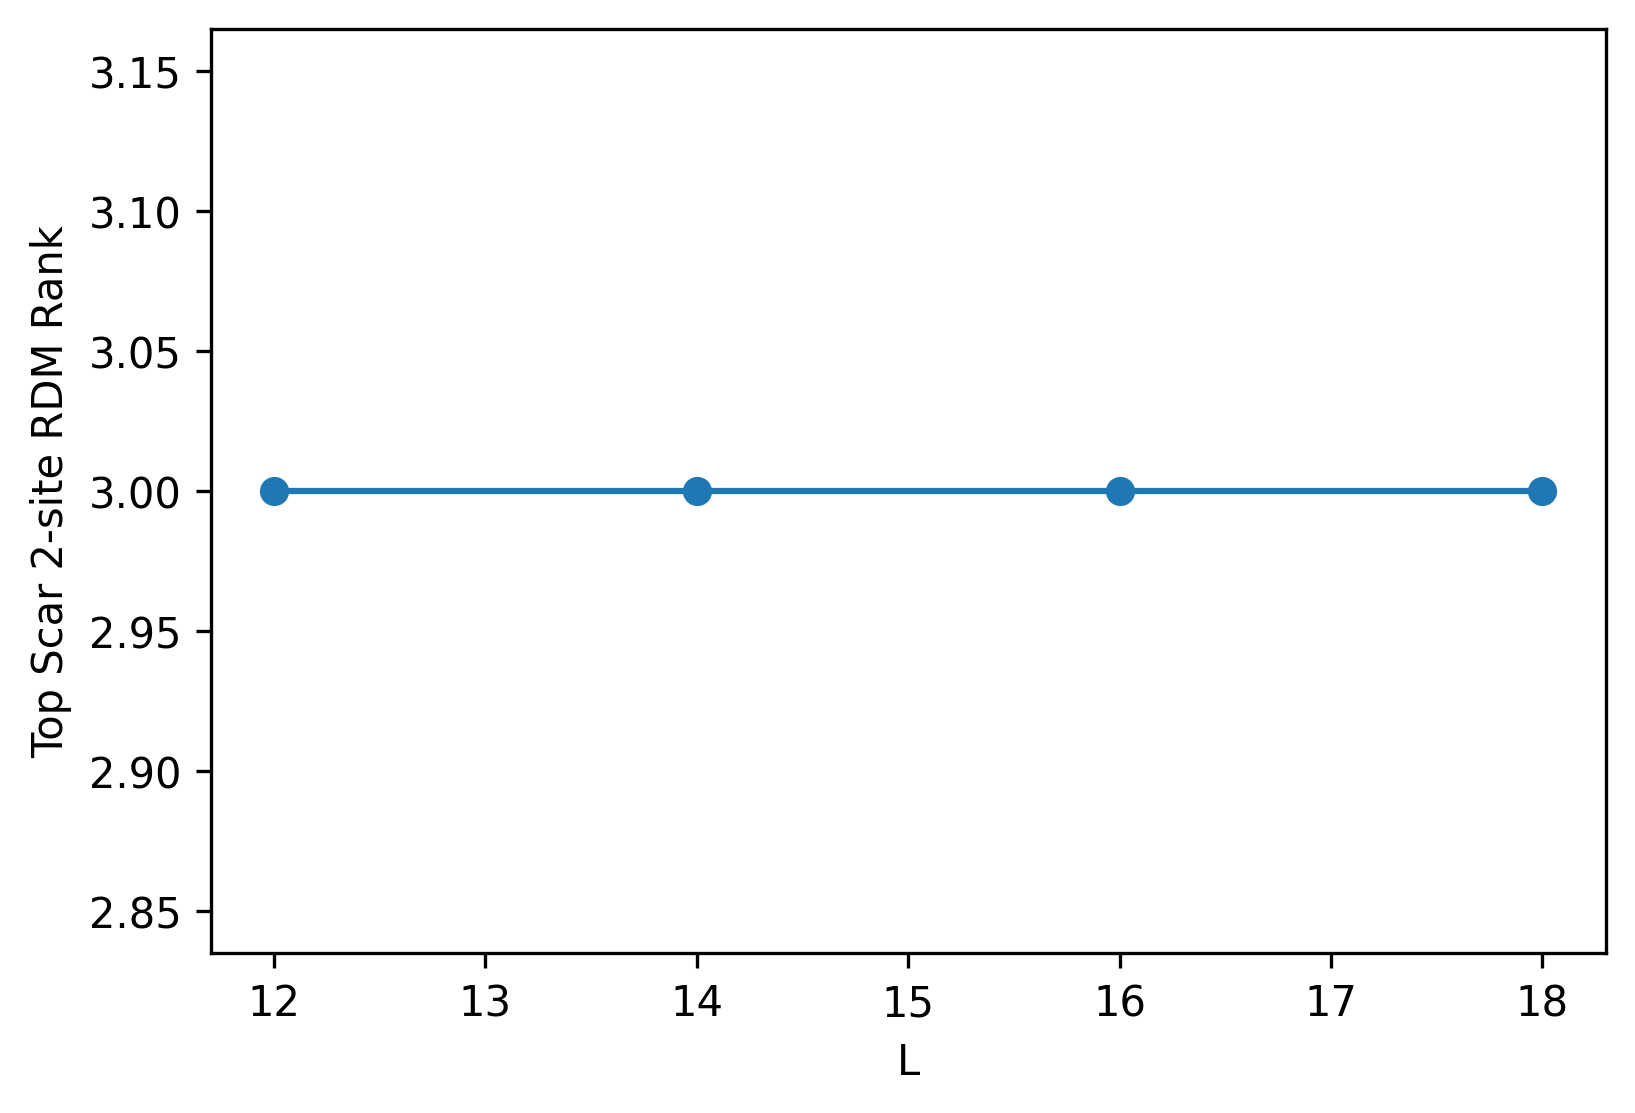
\includegraphics[width=\linewidth]{dw_scar_2.png}
        \caption{}
        \label{fig:image1}
    \end{subfigure}
    % Second image
    \begin{subfigure}{0.45\textwidth}
        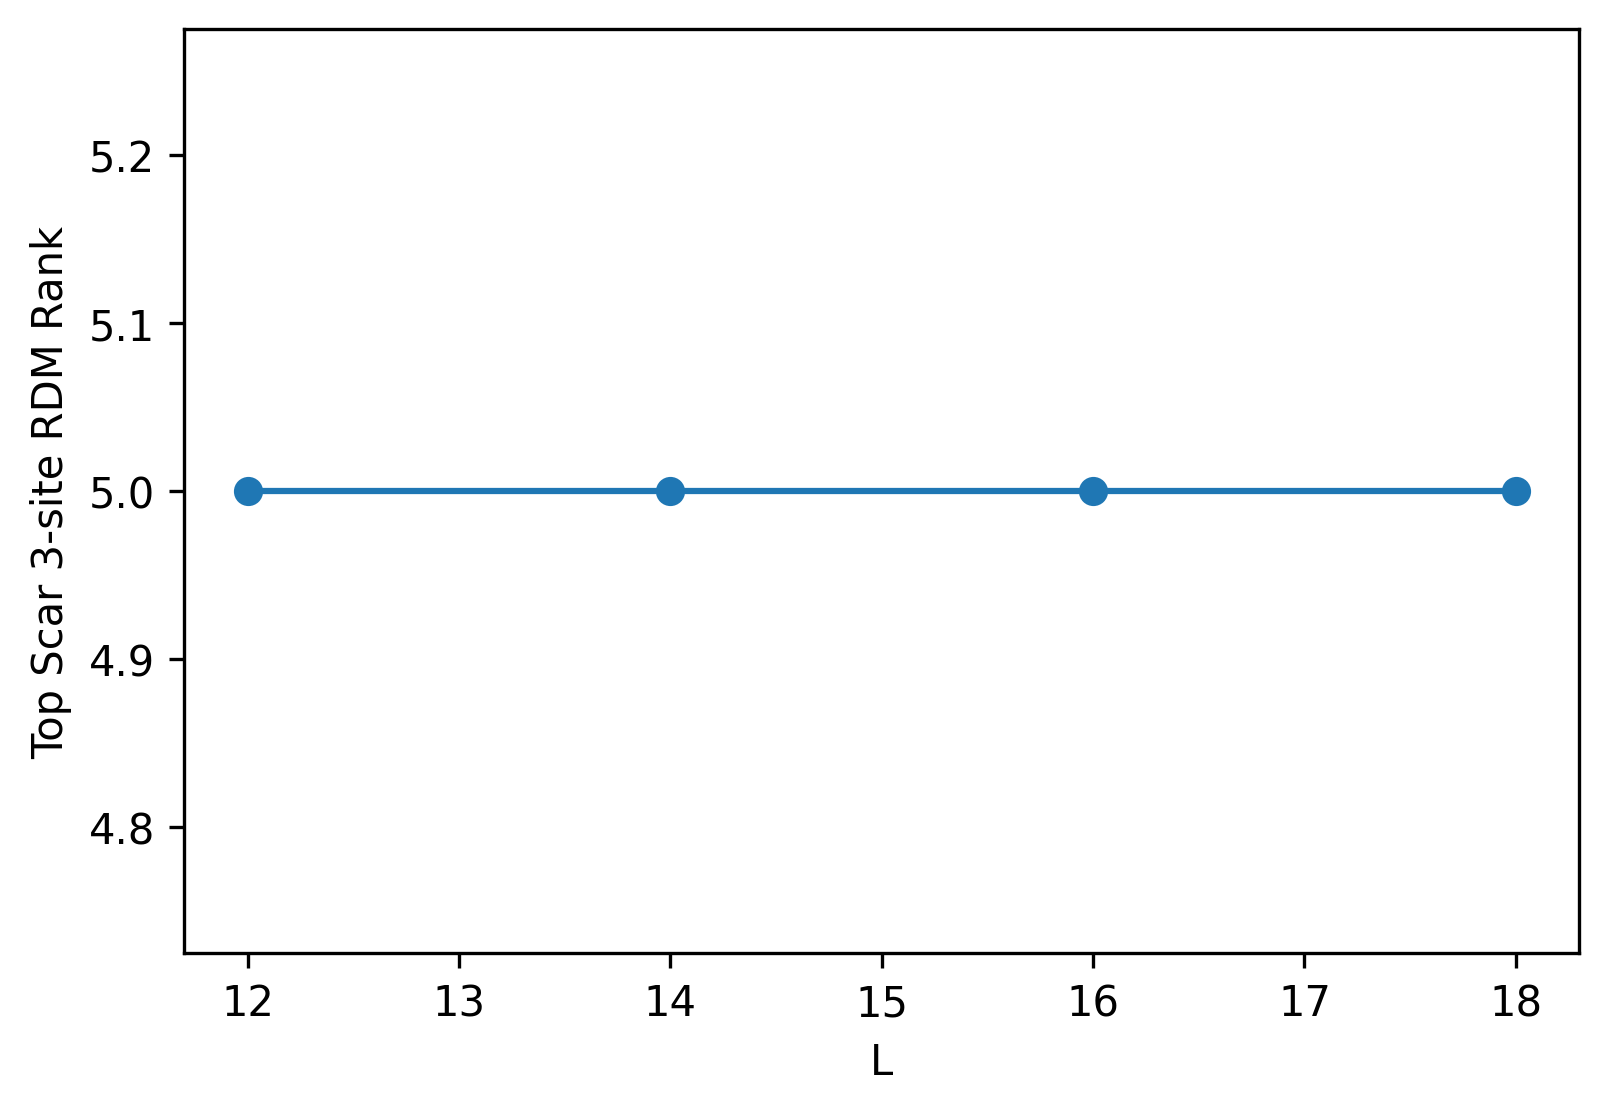
\includegraphics[width=\linewidth]{dw_scar_3.png}
        \caption{}
        \label{fig:image2}
    \end{subfigure}    % Third image
    \begin{subfigure}{0.45\textwidth}
        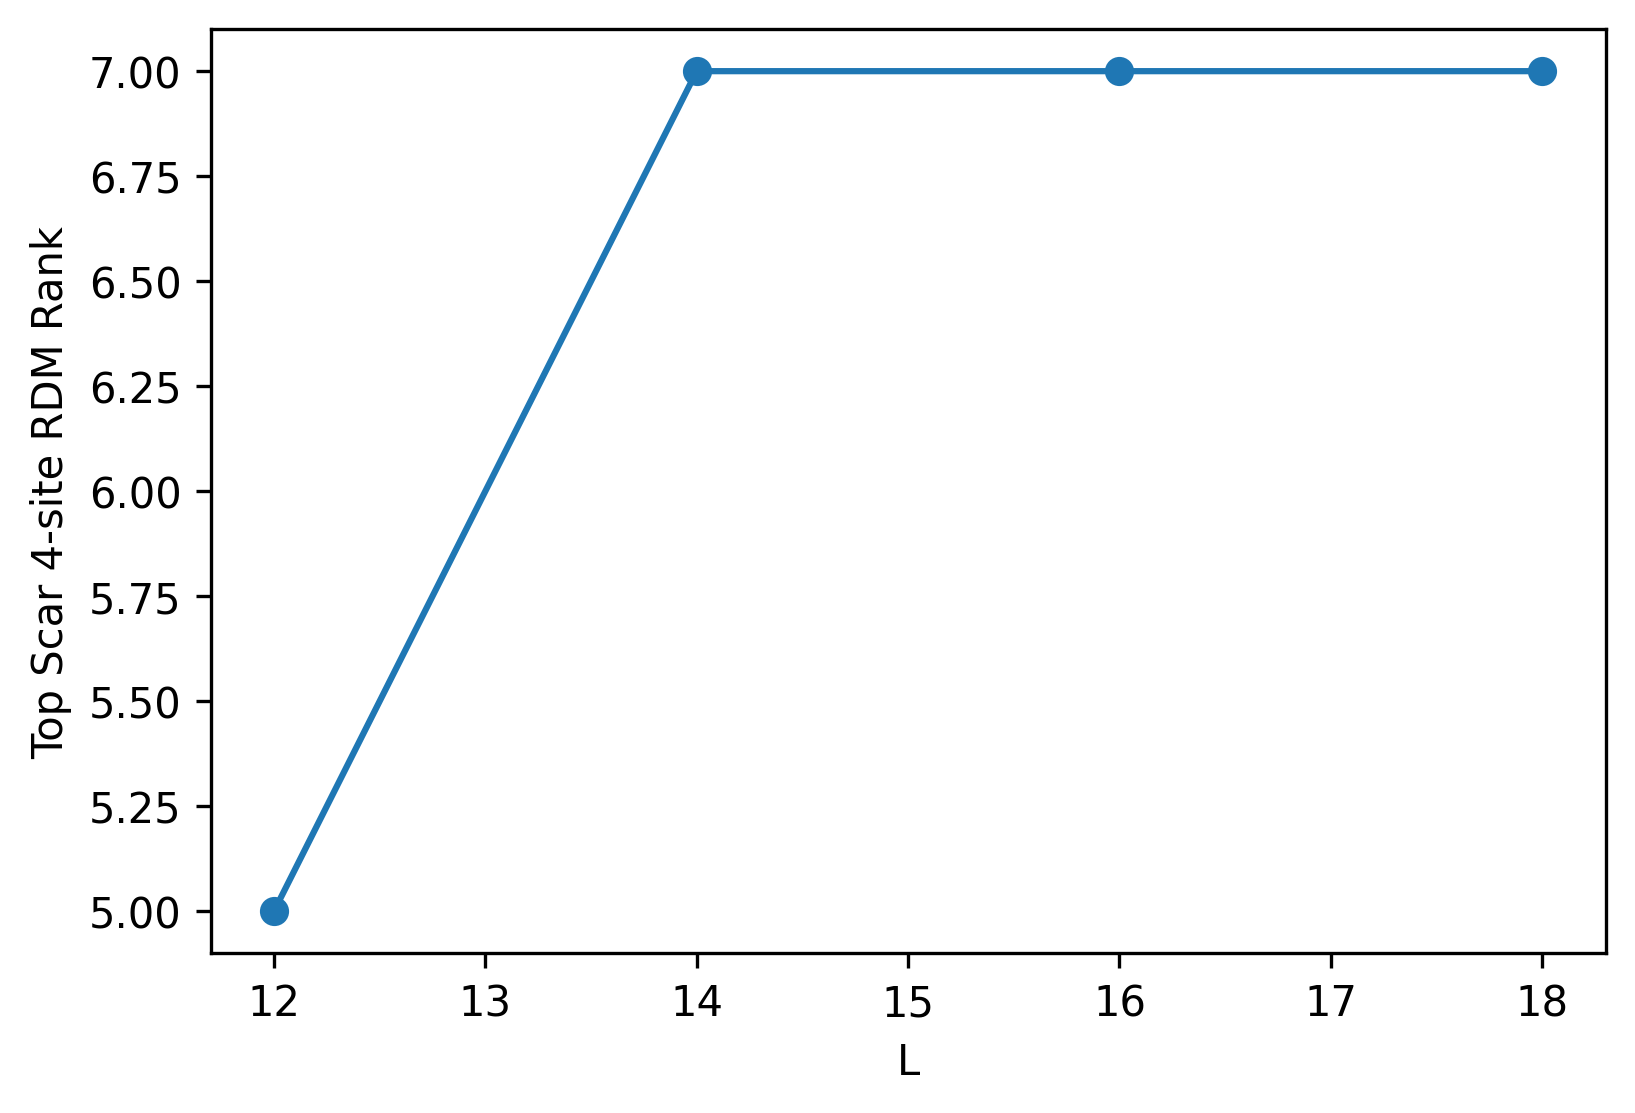
\includegraphics[width=\linewidth]{dw_scar_4.png}
        \caption{}
        \label{fig:image3}
    \end{subfigure}

    % Common caption
    \caption{Innermost 2,3,4-sites RDM  rank (Fig. (a), (b), (c) respectively) of the top scar of the tower $|S_n\rangle$ as a function of increasing $L$.}
    \label{fig:dw_scars_tower}
\end{figure}

\begin{figure}[H]
    \centering
    % First image
    \begin{subfigure}{0.45\textwidth}
        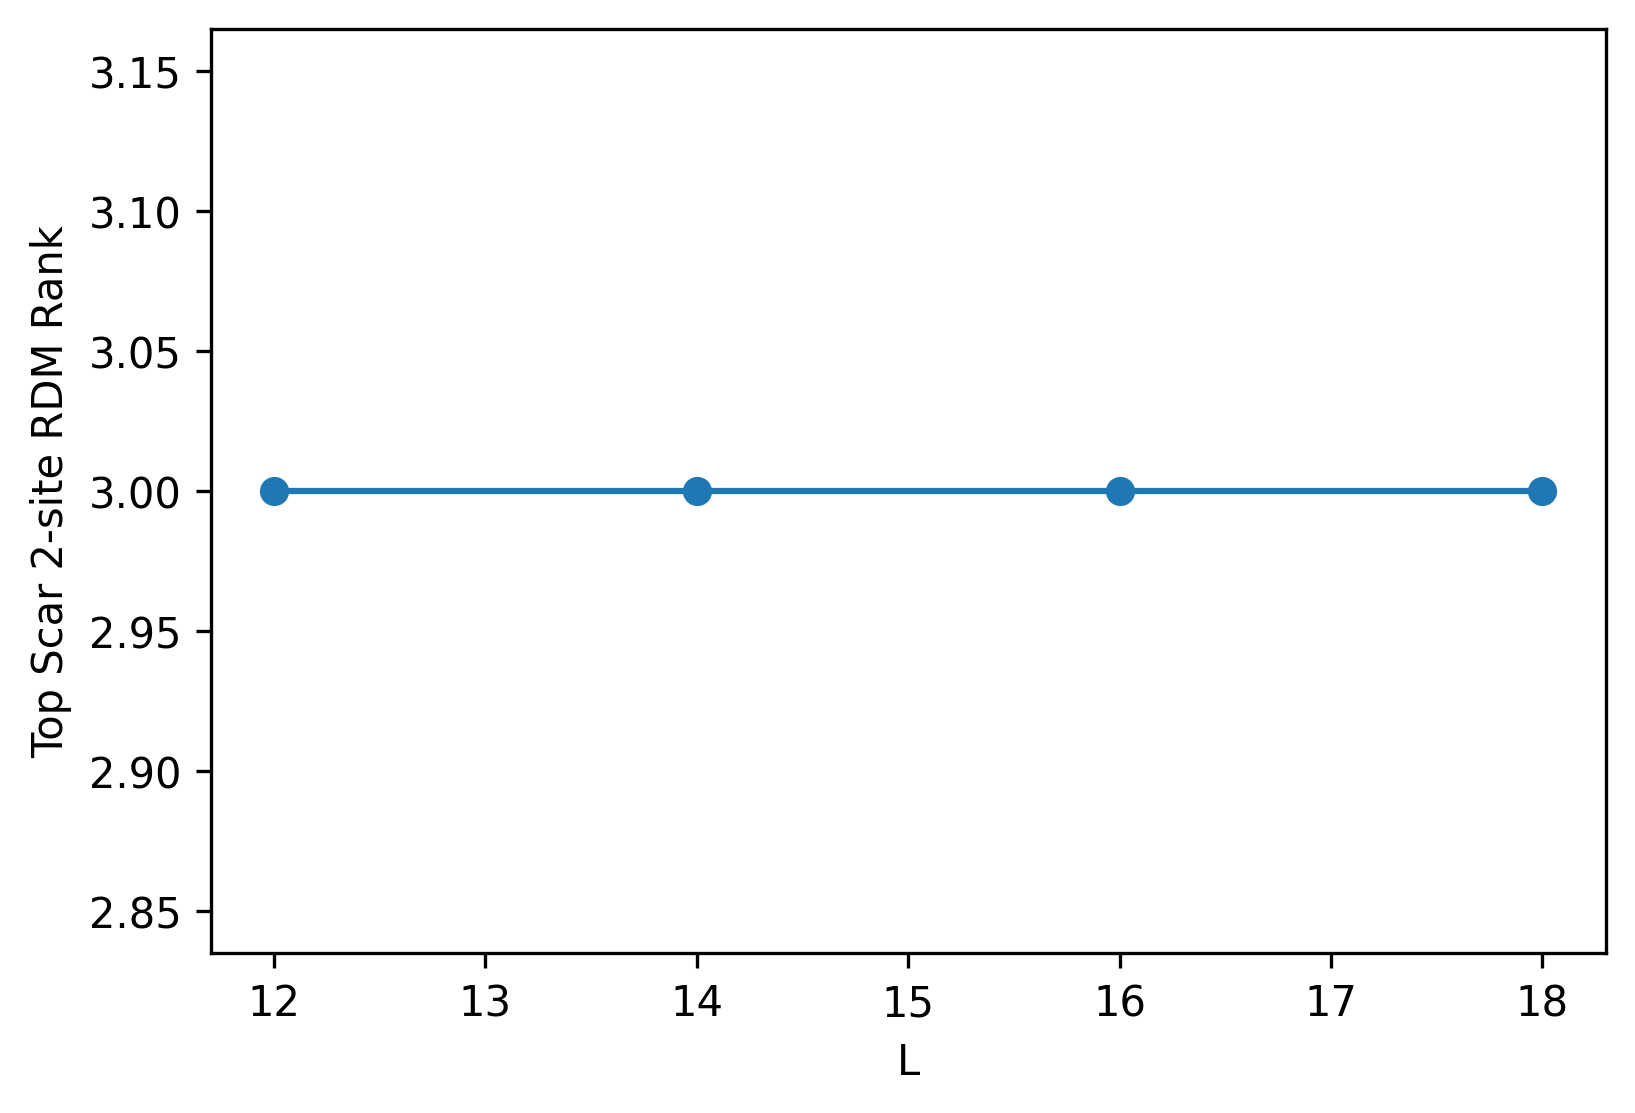
\includegraphics[width=\linewidth]{dw_scar_2p.png}
        \caption{}
        \label{fig:image1p}
    \end{subfigure}
    % Second image
    \begin{subfigure}{0.45\textwidth}
        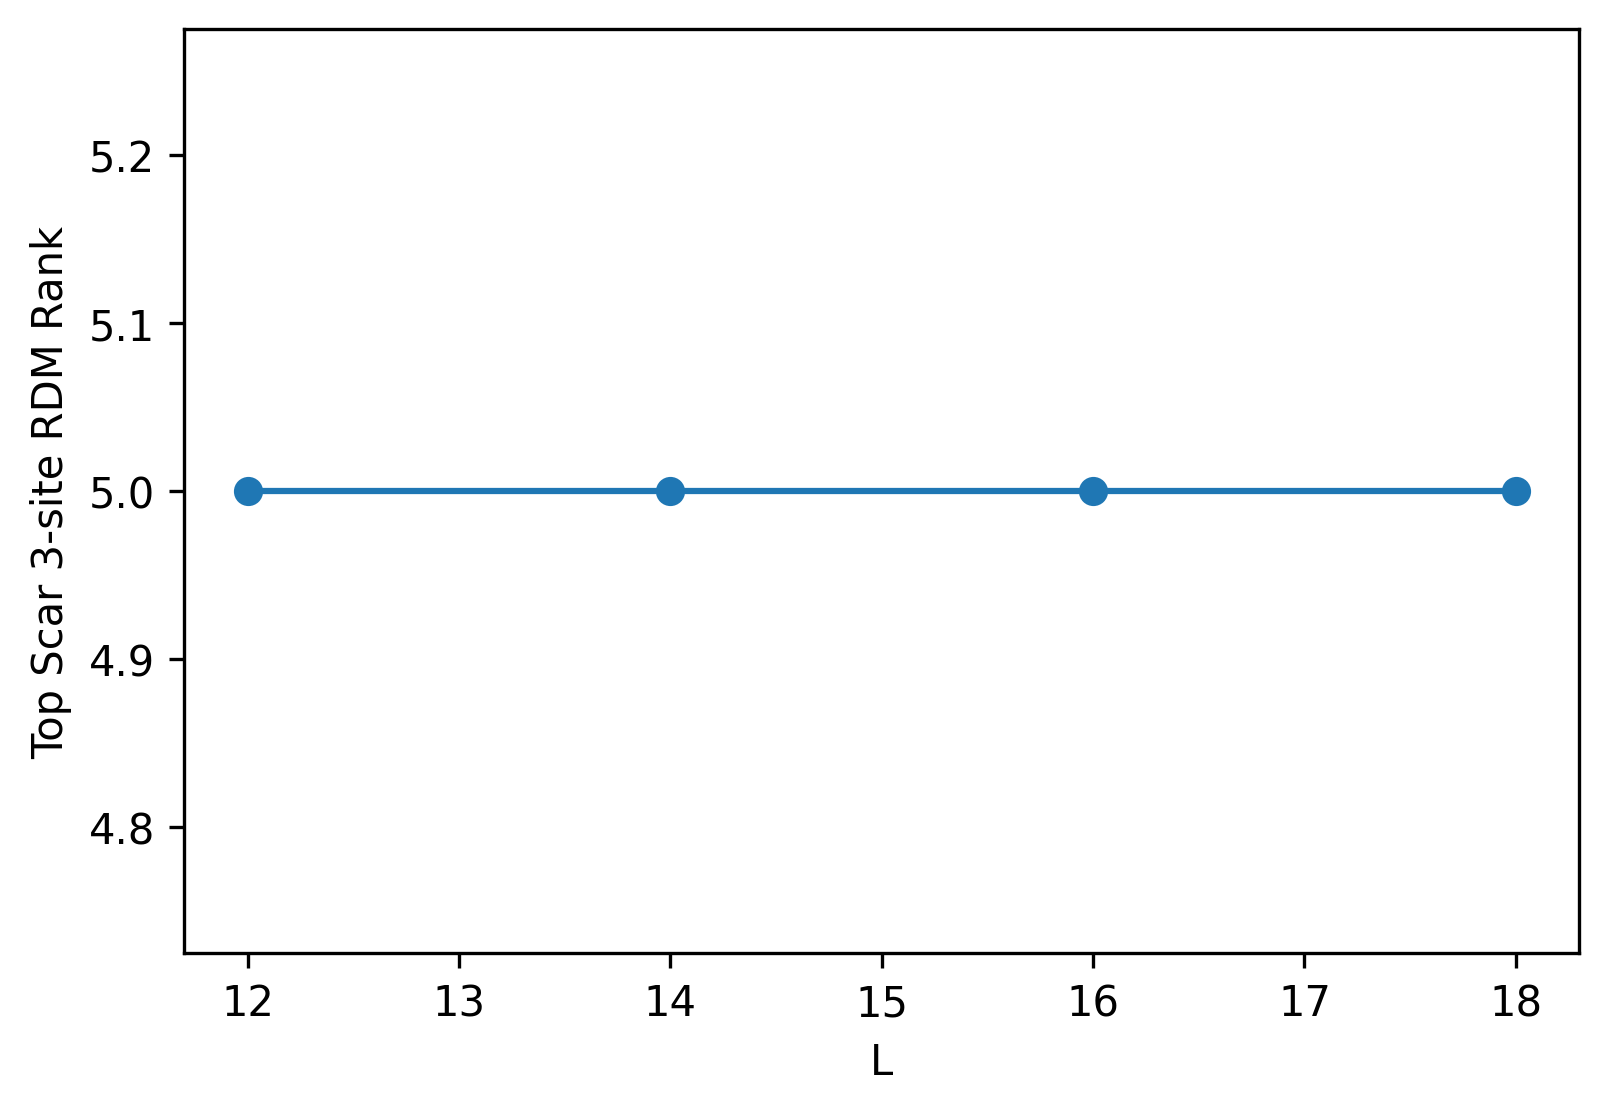
\includegraphics[width=\linewidth]{dw_scar_3p.png}
        \caption{}
        \label{fig:image2p}
    \end{subfigure}    % Third image
    \begin{subfigure}{0.45\textwidth}
        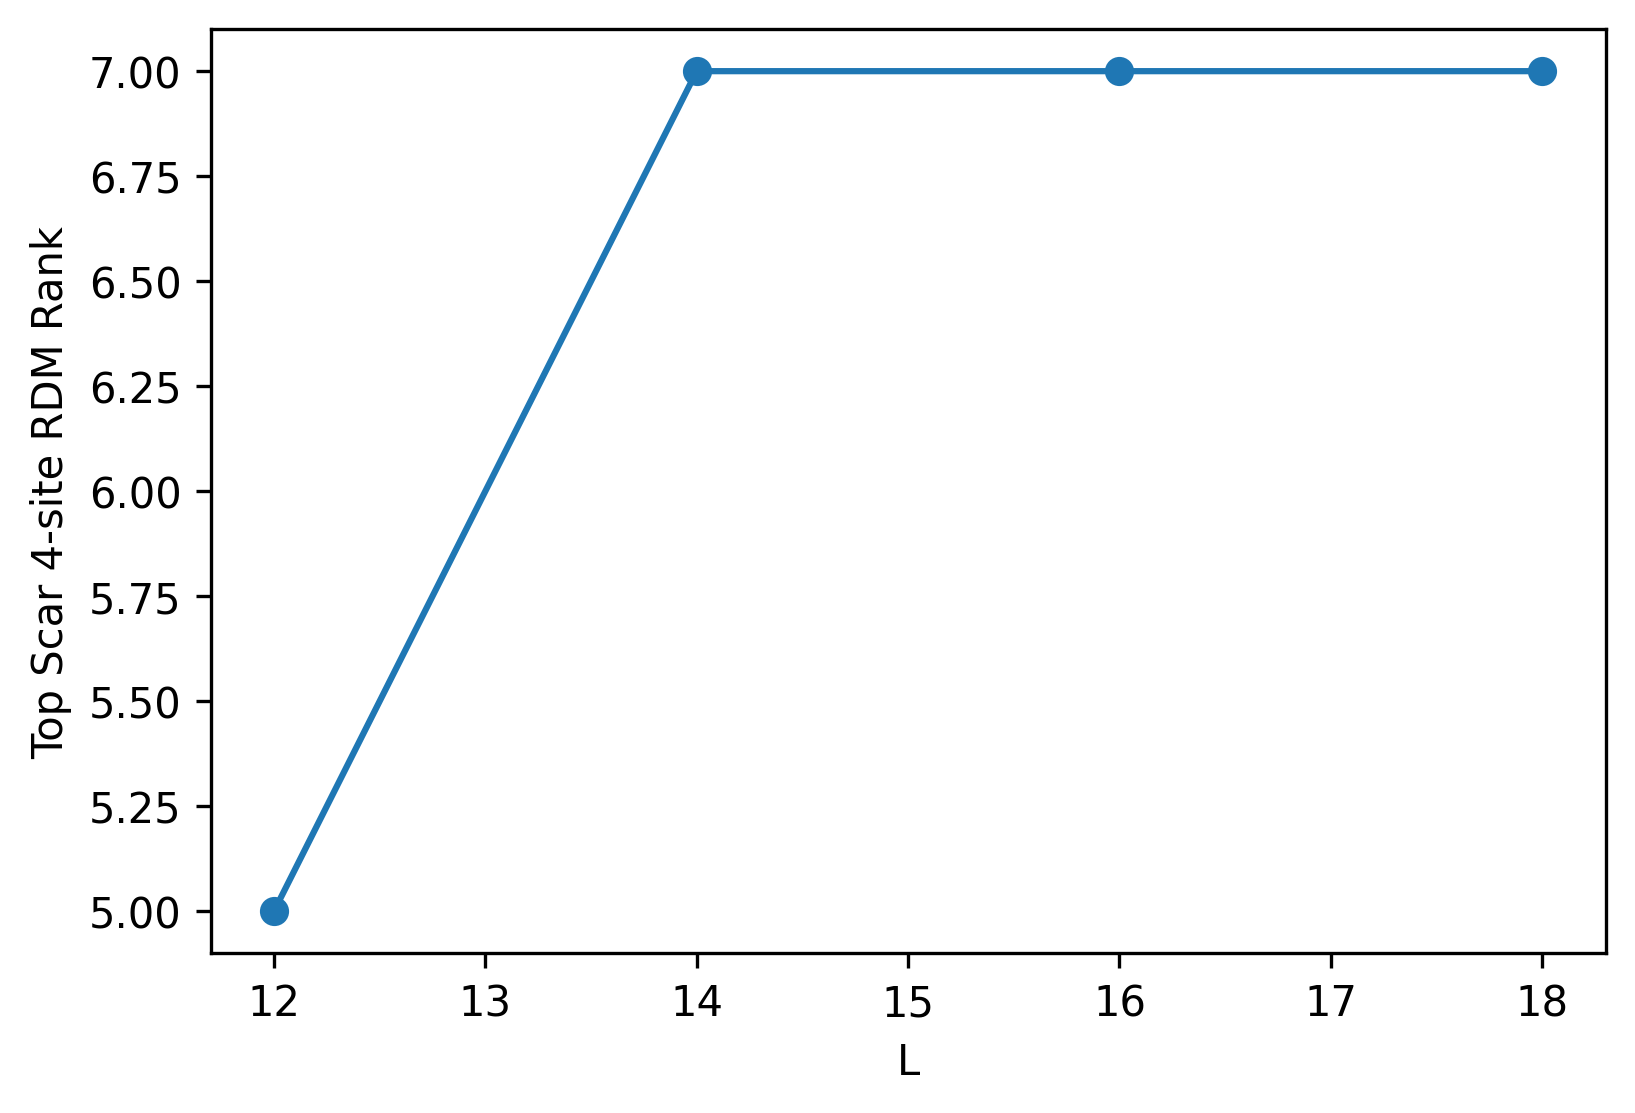
\includegraphics[width=\linewidth]{dw_scar_4p.png}
        \caption{}
        \label{fig:image3p}
    \end{subfigure}

    % Common caption
    \caption{Innermost 2,3,4-sites RDM  rank (Fig. (a), (b), (c) respectively) of the top scar of the tower $|S'_n\rangle$ as a function of increasing $L$.}
    \label{fig:dw_scars_towerp}
\end{figure}


\end{itemize}
\end{itemize}


\vspace{0.3cm}

\section*{3. Spin-1 XY Magnet Tower of Scars}
\begin{itemize}
    \item \textbf{Model:} Spin-1 XY model exhibiting a tower of scarred eigenstates.\\
    The Hamiltonian of the spin-1 XY model is:
	\begin{equation}\label{eqq}
	H = J \sum_{\langle i,j \rangle} \left( S^x_i S^x_j + S^y_i S^y_j \right) 
	+ h \sum_i S^z_i + D \sum_i \left(S^z_i\right)^2,
	\end{equation}
	
	where $S^\alpha_i$ ($\alpha = x, y, z$) are spin-1 operators defined on the sites of a 1-dimensional chain of length L, and $\langle i,j \rangle$ denotes nearest neighbors.  

	
    \item \textbf{Reference:} \href{https://journals.aps.org/prl/abstract/10.1103/PhysRevLett.123.147201}{Phys. Rev. Lett. 123, 147201 (2019)}.
    \item \textbf{Analysis:}
    \begin{itemize}
        \item Focused on exact scarred states with known analytic forms.\\ There are two towers of scars, both of length $L+1$.\\
    The first tower is described by:
	    \begin{equation}
	|S_n\rangle = \mathcal{N}(L, n) \left(J^\dagger\right)^n |\Omega\rangle, \quad n = 0,\hdots,L
	\end{equation}
	
	where $|\Omega\rangle = \bigotimes_i \left| m_i = -1 \right\rangle$ and $\mathcal{N}(L, n) = \sqrt{(L-n)!/n!L!}\,$. $J^\dagger$ is the ladder operator, defined as:
	
	\begin{equation}
	J^\dagger = \frac{1}{2}\sum_{i=1}^{L} (-1)^i \left(S^+_i\right)^2, 
	\end{equation}
	
	where $S_i^\pm = S_i^x \pm i S_i^y$.\\
     The second tower is given by 
     \begin{equation}
	|S'_n\rangle \propto \sum_{i_1 \neq \hdots \neq i_n} (-1)^{i_1 + \hdots + i_n} \left(S^+_{i_1}S^+_{i_1+1}\right)\hdots\left(S^+_{i_n}S^+_{i_n+1}\right)  |\Omega\rangle, \quad n = 0,\hdots,L
	\end{equation}
	Both scar towers are annihilated by the first term of \eqref{eqq}, which breaks what is known as Q-SU(2) symmetry (a special SU(2) symmetry that only scars have - see the reference \href{https://arxiv.org/pdf/2007.16207}{https://arxiv.org/pdf/2007.16207} for explanation): $J \sum_{\langle i,j \rangle} \left( S^x_i S^x_j + S^y_i S^y_j \right)  |S_n\rangle = J \sum_{\langle i,j \rangle} \left( S^x_i S^x_j + S^y_i S^y_j \right)  |S'_n\rangle = 0$.
        \item Entanglement entropy computed and compared with theoretical values.
        Only $|S_5\rangle$ for L=10 sites was considered (with OBC!)
        
         \begin{equation}
        S^{\,|S_5\rangle}_A \approx 1.23 \approx \frac{1}{2} \ln \left(\frac{e \pi 10}{8}\right)
        \end{equation}
        
        For generic $L$, $S^{\,|S_5\rangle}_A$ scales logarithmically with system size, i.e. $S^{\,|S_5\rangle}_A = \frac{1}{2} \ln \left(\frac{e \pi L}{8}\right)$. Because $S^{\,|S_5\rangle}_A$ is at the top of the tower - it has maximum possible 						value of entanglement entropy among the scars - we can assume that all scars have sub-volume scaling with system size, i.e. constant or at most logarithmic.
        
        \item Evaluated ranks of 2- to 4-site adjacent RDMs.
         \begin{table}[H]
	\centering
	\begin{tabular}{|c|ccc|}
	\hline
	\textbf{$|S_n\rangle$} & \multicolumn{3}{c|}{\textbf{RDM Rank}} \\
	\cline{2-4}
	& \textbf{2-sites} & \textbf{3-sites} & \textbf{4-sites}\\
	\hline
	 n = 0 & 1 & 1 & 1 \\
	 n = 1 & 2 & 2 & 2 \\
	 n = 2 & 3 & 3 & 3 \\
	 n = 3 & 3 & 4 & 4 \\
	 n = 4 & 3 & 4 & 5 \\  
	 n = 5 & 3 & 4 & 5 \\
	 n = 6 & 3 & 4 & 5 \\
	 n = 7 & 3 & 4 & 4 \\
	 n = 8 & 3 & 3 & 3 \\
	 n = 9 & 2 & 2 & 2 \\
	 n = 10 & 1 & 1 & 1 \\
	\hline
	\end{tabular}
	\caption{RDM ranks for 2, 3, and 4 adjacent sites in the $|S_n\rangle$ scar tower for $L=10$.}
	\label{tab:ranks21}
	\end{table}

	 \begin{table}[H]
	\centering
	\begin{tabular}{|c|ccc|}
	\hline
	\textbf{$|S'_n\rangle$} & \multicolumn{3}{c|}{\textbf{RDM Rank}} \\
	\cline{2-4}
	& \textbf{2-sites} & \textbf{3-sites} & \textbf{4-sites} \\
	\hline
          n = 0 & 1 & 1 & 1 \\
	 n = 1 & 4 & 4 & 4 \\
	 n = 2 & 6 & 8 & 8 \\
	 n = 3 & 7 & 11 & 12 \\
	 n = 4 & 7 & 12 & 15 \\  
	 n = 5 & 7 & 12 & 16 \\
	 n = 6 & 7 & 12 & 15 \\
	 n = 7 & 7 & 11 & 12 \\
	 n = 8 & 6 & 8 & 8 \\
	 n = 9 & 4 & 4 & 4 \\
	 n = 10 & 1 & 1 & 1 \\
	\hline
	\end{tabular}
	\caption{RDM ranks for 2, 3, and 4 adjacent sites in the $|S'_n\rangle$ scar tower for $L=10$.\\ \textbf{The scars $|S'_n\rangle$ are less rank-deficient than the $|S_n\rangle$ scars}.}
	\label{tab:ranks22}
	\end{table}
	
	\begin{figure}[H]
    \centering
    % First image
    \begin{subfigure}{0.45\textwidth}
        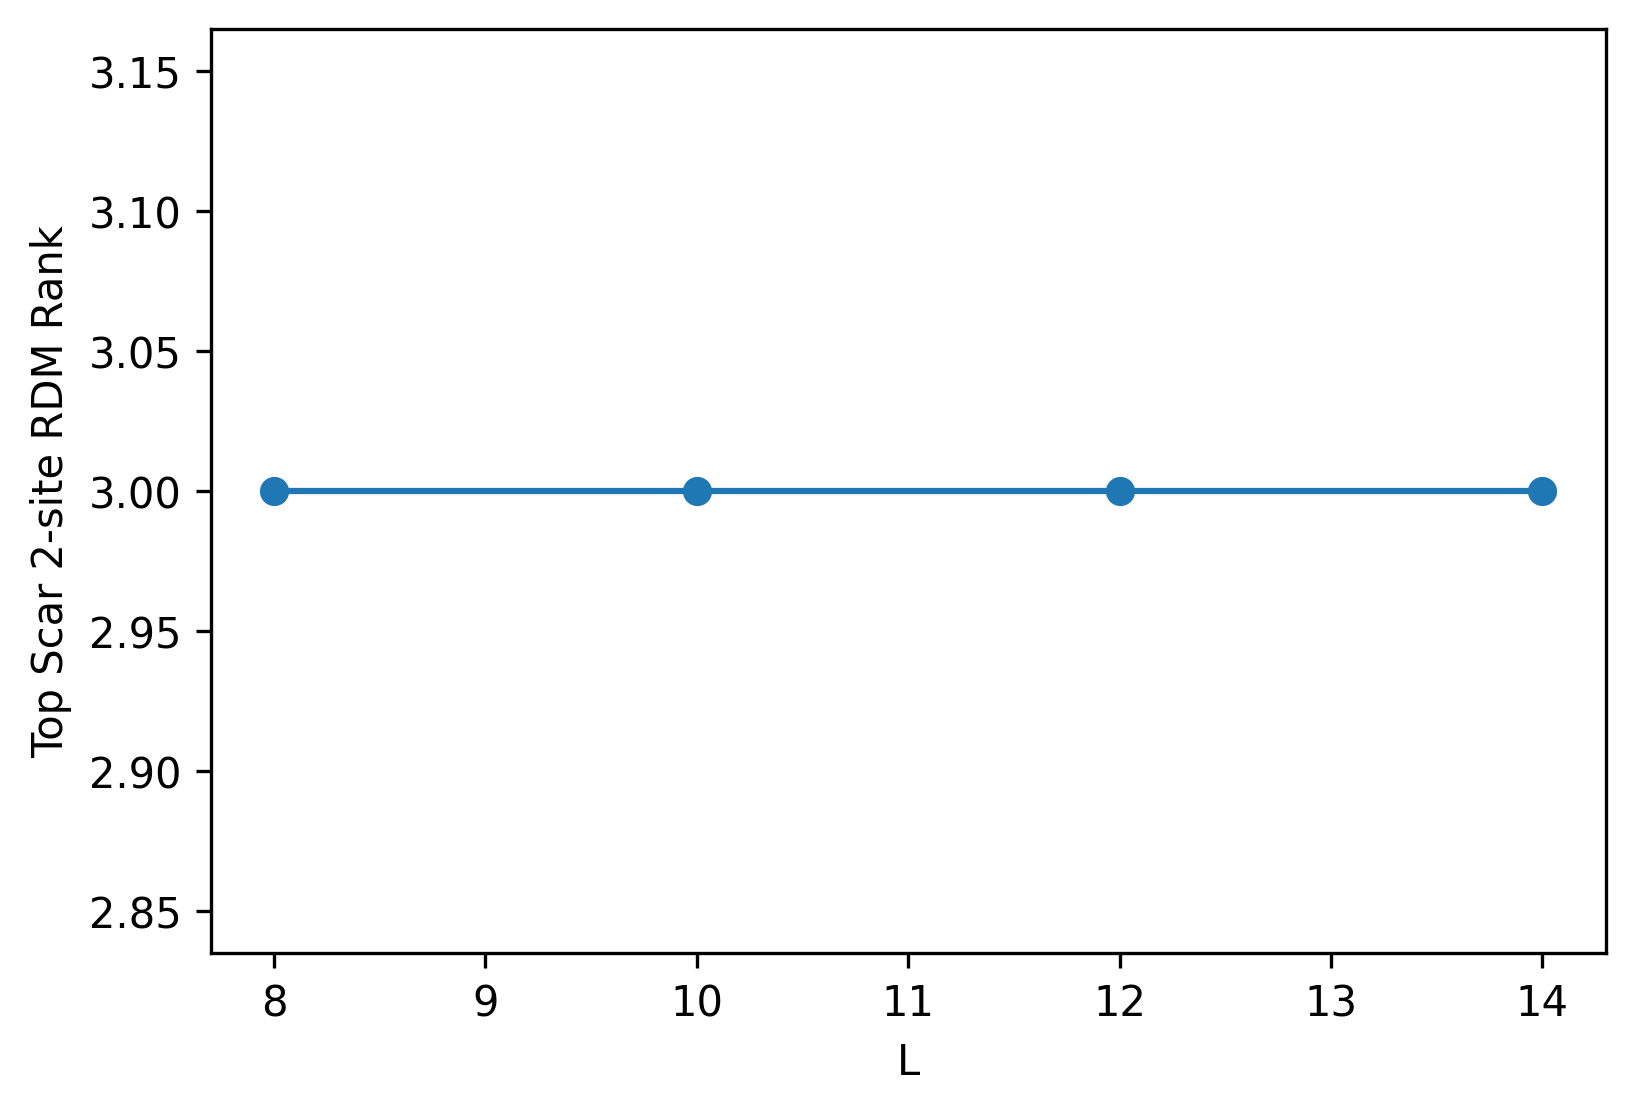
\includegraphics[width=\linewidth]{xy_scar_2.png}
        \caption{}
        \label{fig:image1xy}
    \end{subfigure}
    % Second image
    \begin{subfigure}{0.45\textwidth}
        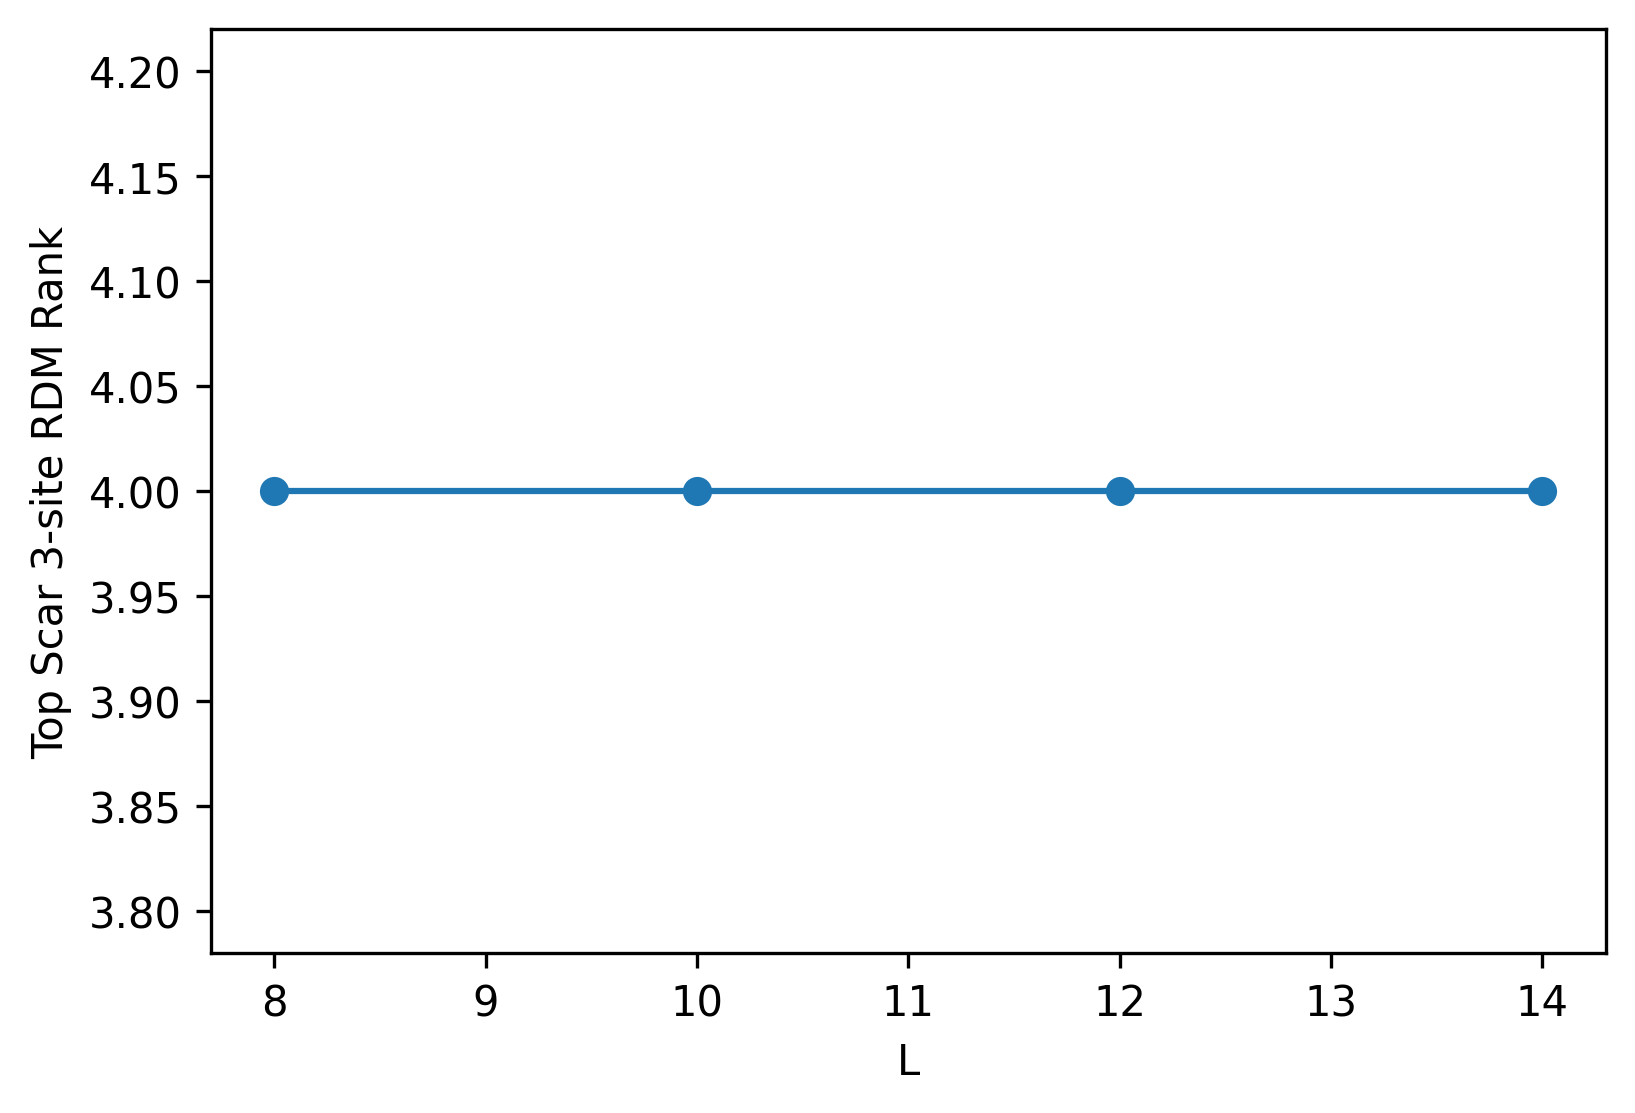
\includegraphics[width=\linewidth]{xy_scar_3.png}
        \caption{}
        \label{fig:image2xy}
    \end{subfigure}    % Third image
    \begin{subfigure}{0.45\textwidth}
        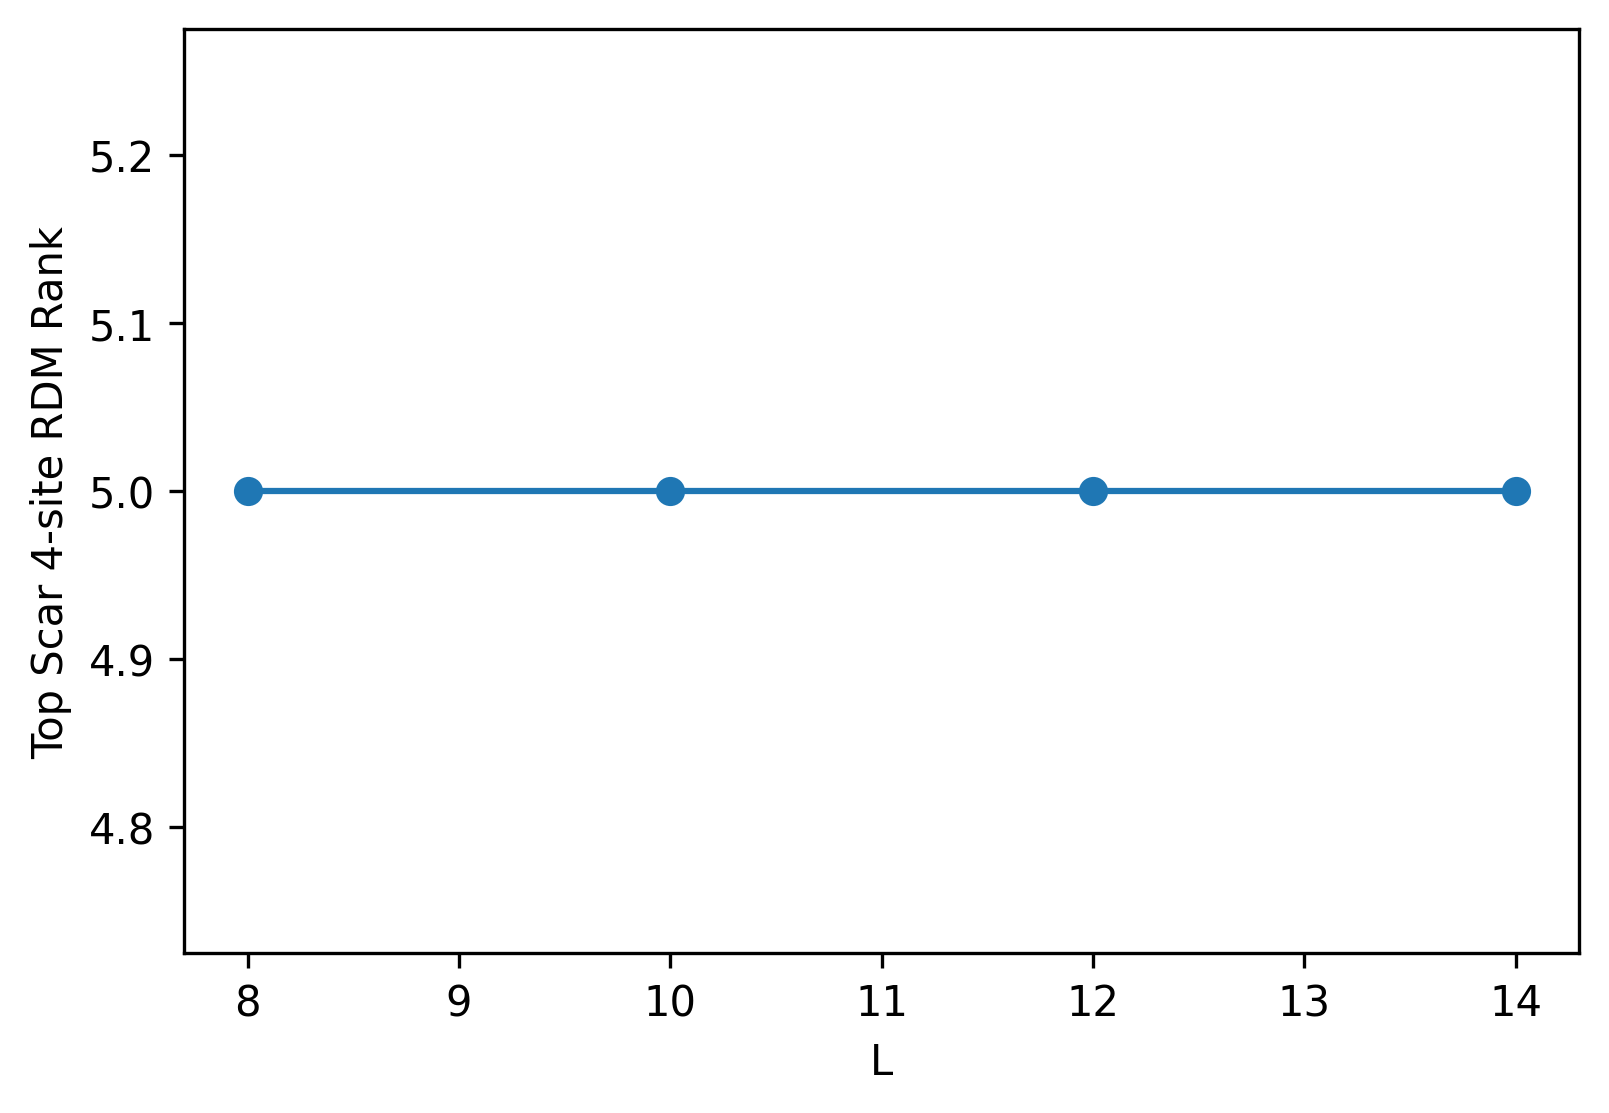
\includegraphics[width=\linewidth]{xy_scar_4.png}
        \caption{}
        \label{fig:image3xy}
    \end{subfigure}

    % Common caption
    \caption{Innermost 2,3,4-sites RDM  rank (Fig. (a), (b), (c) respectively) of the top scar of the tower $|S_n\rangle$ as a function of increasing $L$.}
    \label{fig:xy_scars_tower}
\end{figure}

\begin{figure}[H]
    \centering
    % First image
    \begin{subfigure}{0.45\textwidth}
        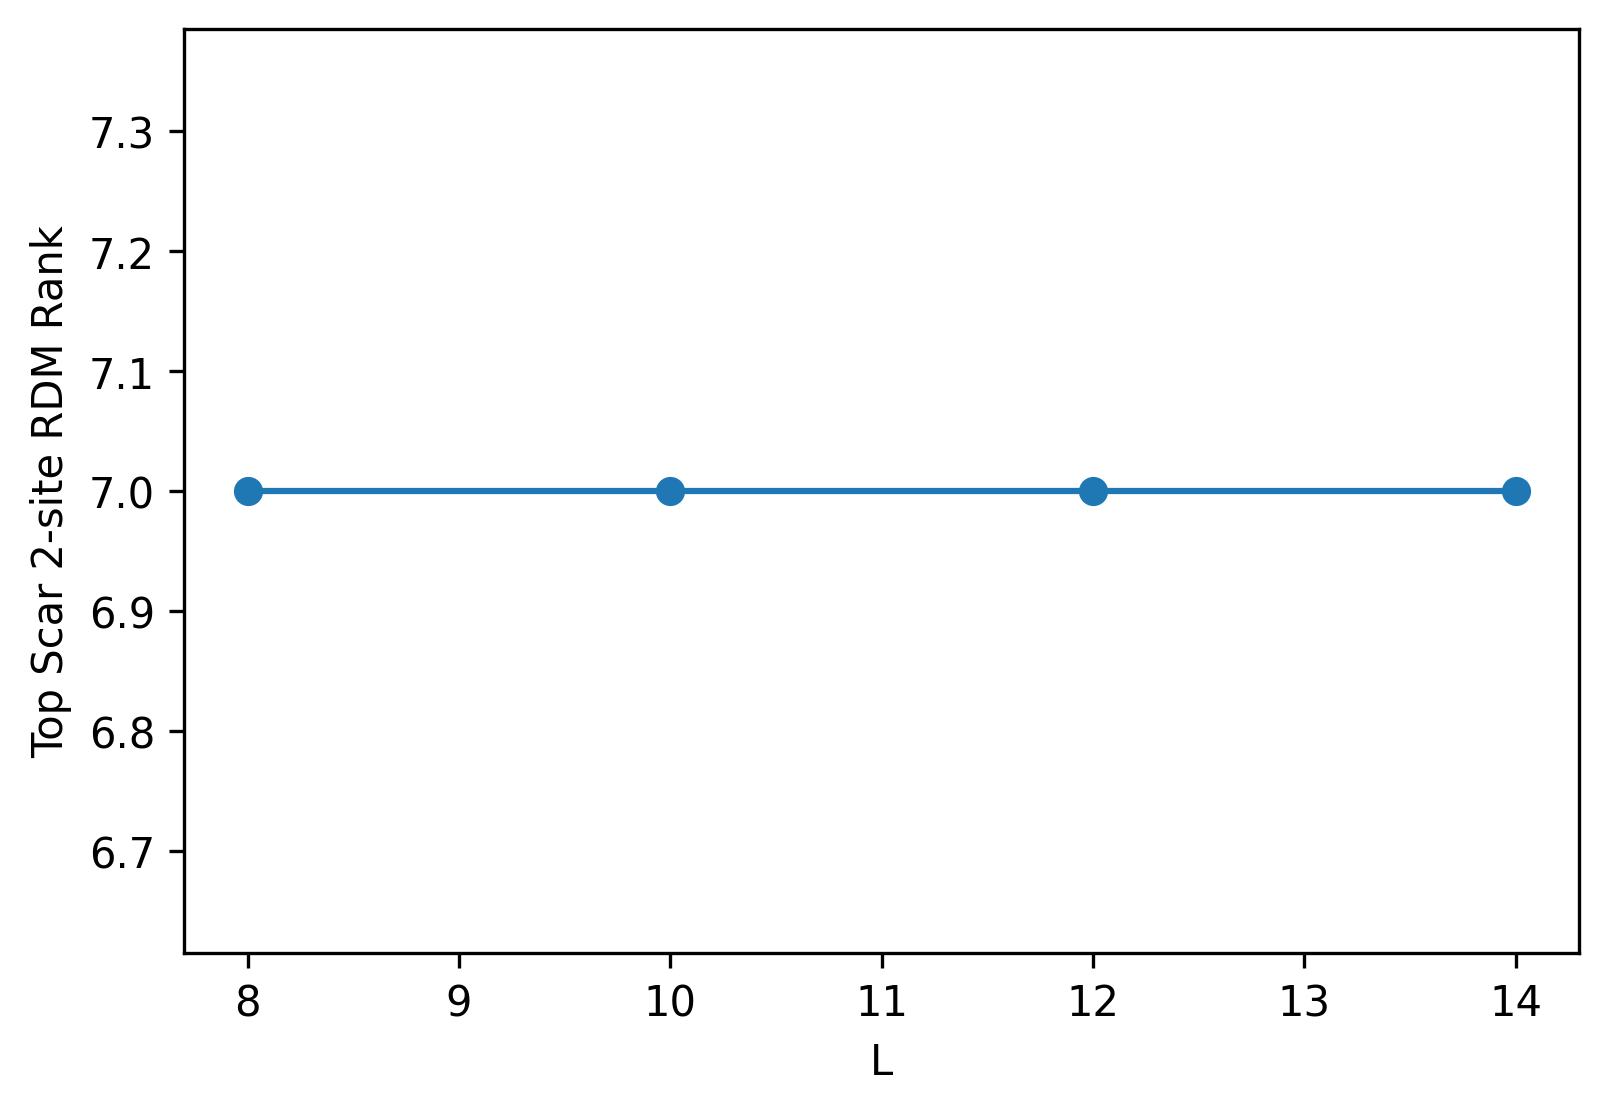
\includegraphics[width=\linewidth]{xy_scar_2p.png}
        \caption{}
        \label{fig:image1pxy}
    \end{subfigure}
    % Second image
    \begin{subfigure}{0.45\textwidth}
        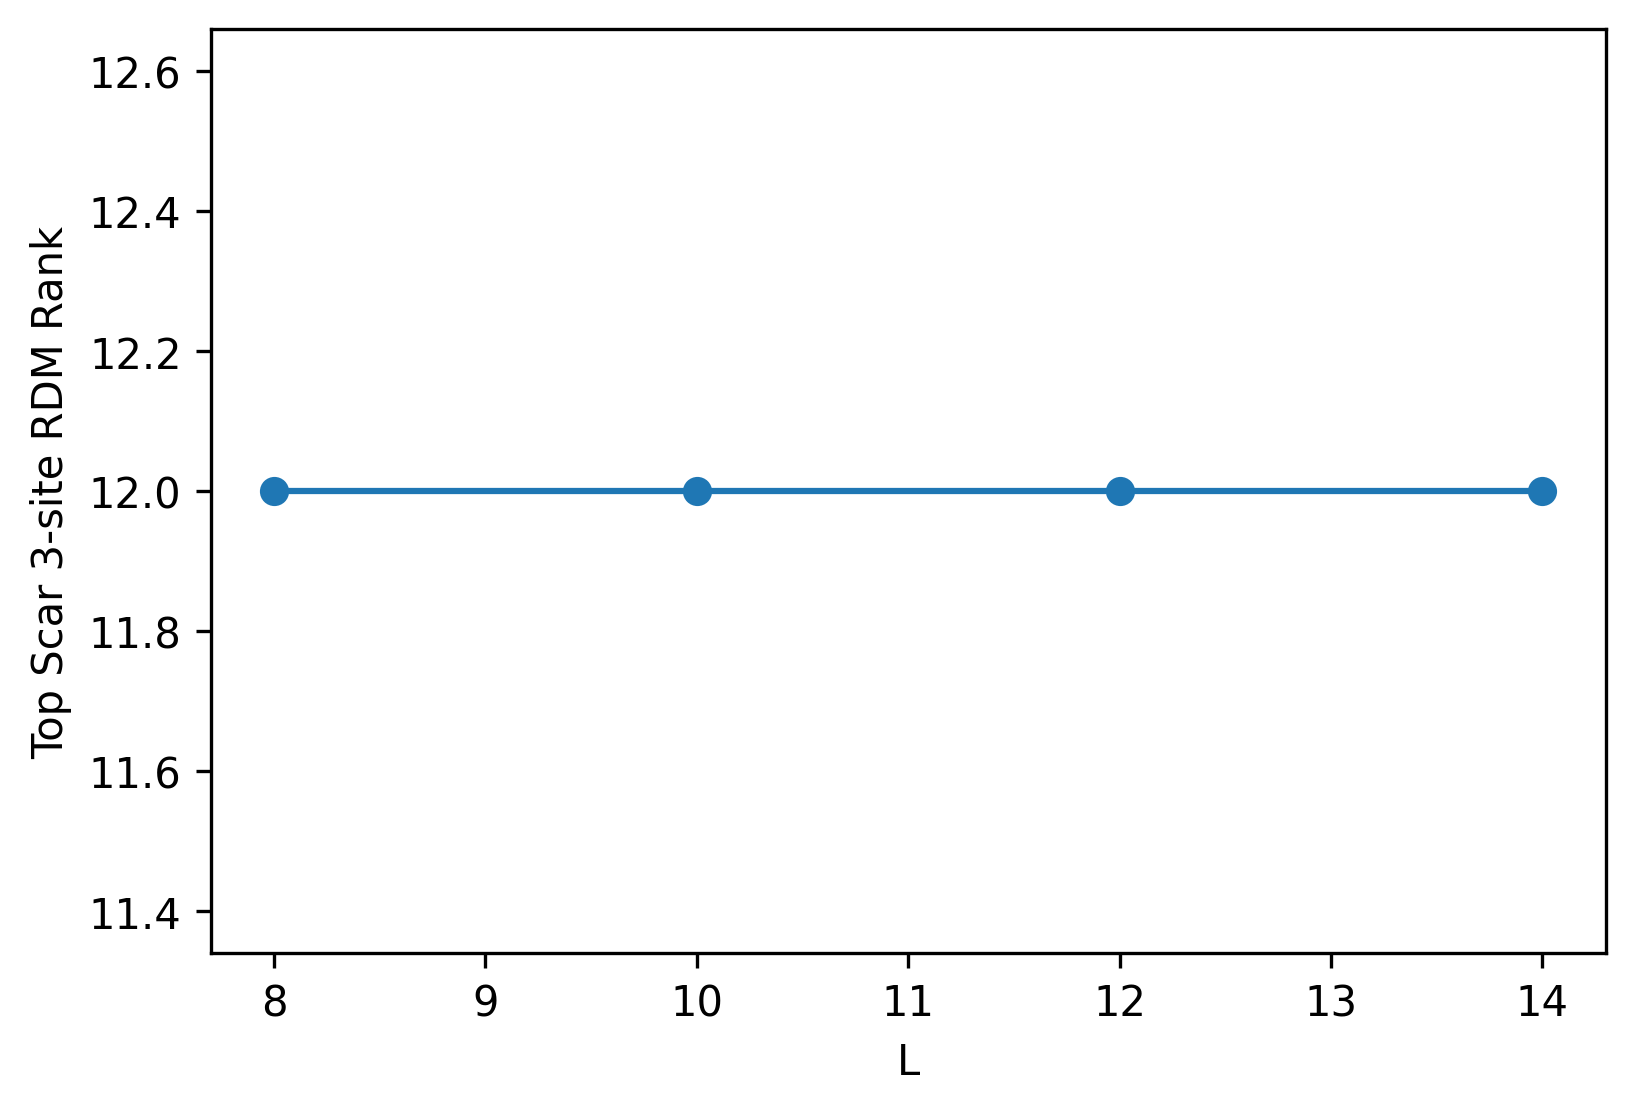
\includegraphics[width=\linewidth]{xy_scar_3p.png}
        \caption{}
        \label{fig:image2pxy}
    \end{subfigure}    % Third image
    \begin{subfigure}{0.45\textwidth}
        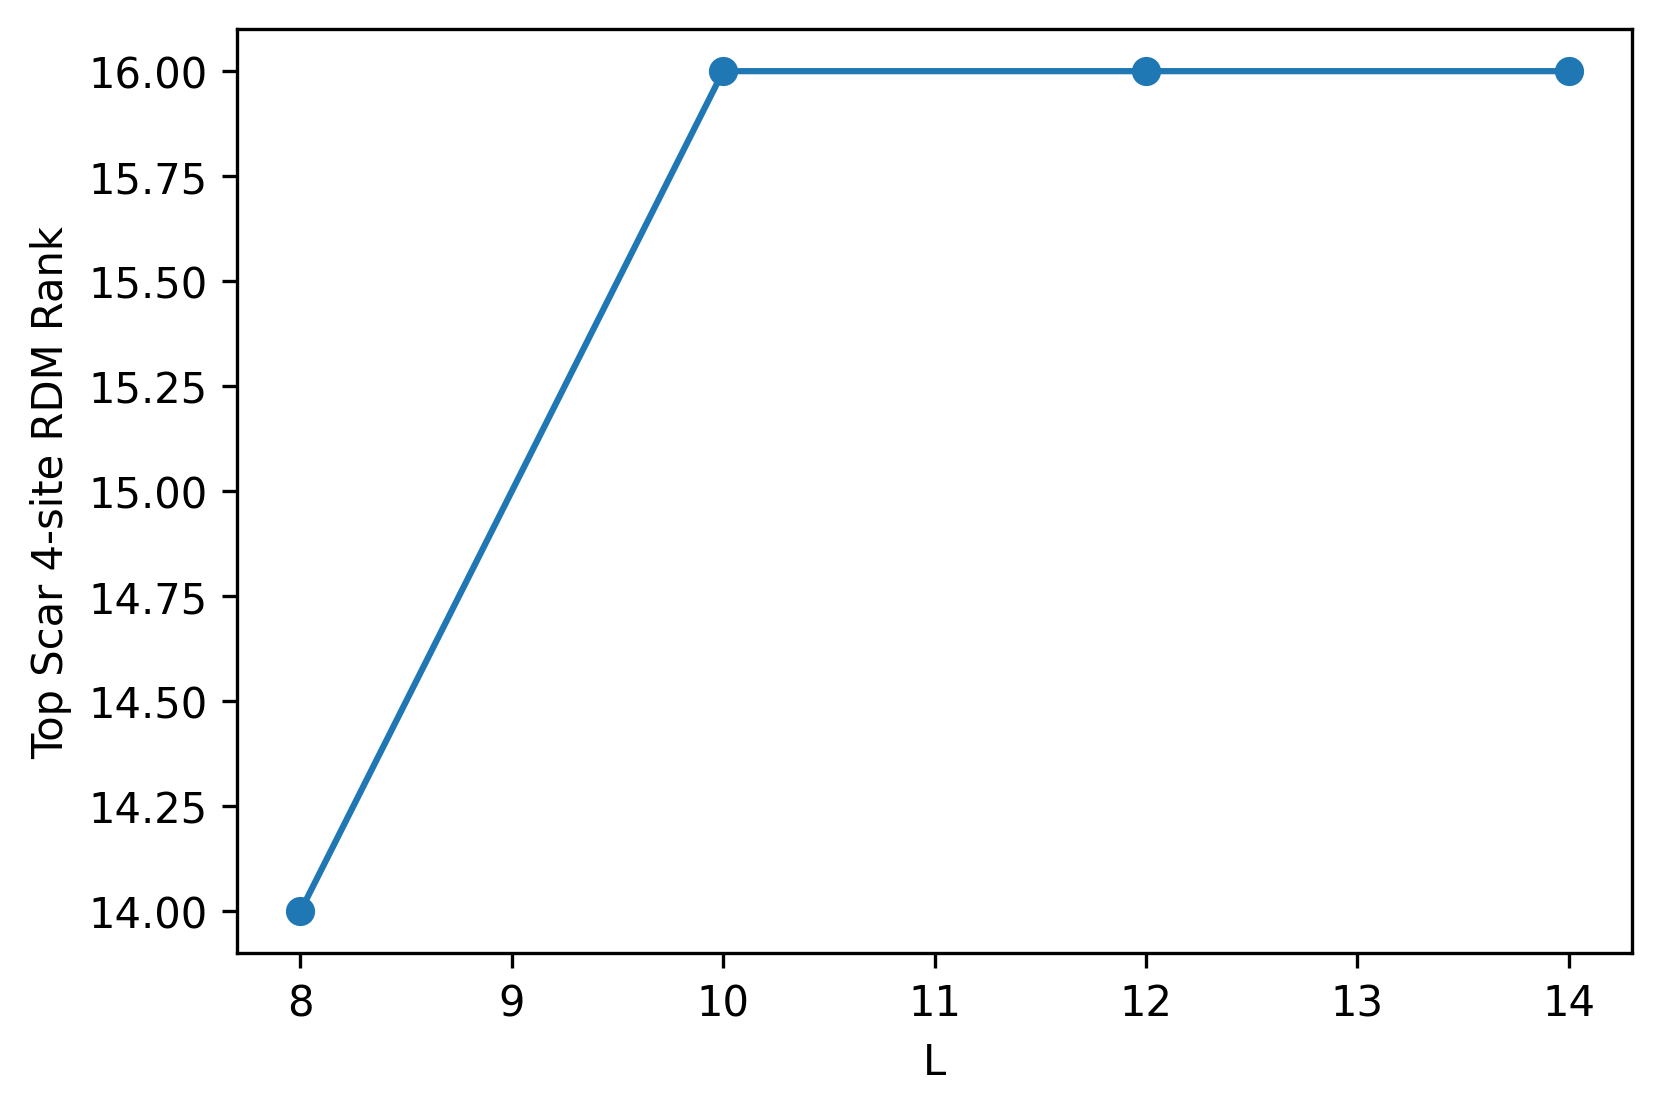
\includegraphics[width=\linewidth]{xy_scar_4p.png}
        \caption{}
        \label{fig:image3pxy}
    \end{subfigure}

    % Common caption
    \caption{Innermost 2,3,4-sites RDM  rank (Fig. (a), (b), (c) respectively) of the top scar of the tower $|S'_n\rangle$ as a function of increasing $L$.}
    \label{fig:xy_scars_towerp}
\end{figure}

    \end{itemize}
    \end{itemize}
       
\vspace{0.3cm}

\section*{4. Hubbard/Hirsch $\eta$-pairing Tower of Scars}
\begin{itemize}
  \item \textbf{Model:} 1D fermionic lattice model with on-site interactions and bond-charge coupling, known as the Hirsch model. The Hamiltonian is written as:
    \begin{equation}
    H = H_{\text{Hubbard}} + H_{\text{Hirsch}},
    \end{equation}
    where
    \begin{align}
    H_{\text{Hubbard}} &= - t \sum_{\langle i, j \rangle, \sigma} \left( c^\dagger_{i\sigma} c_{j\sigma} + \text{h.c.} \right) + U \sum_i n_{i\uparrow} n_{i\downarrow} - \mu \sum_{i, \sigma} n_{i\sigma}, \\
    H_{\text{Hirsch}} &= X \sum_{\langle i, j \rangle, \sigma} \left( n_{i\bar{\sigma}} + n_{j\bar{\sigma}} \right) \left( c^\dagger_{i\sigma} c_{j\sigma} + \text{h.c.} \right),
    \end{align}
    and \( X \in \mathbb{R} \) is the Hirsch parameter that controls the strength of the bond-charge interaction. Here, \( c^\dagger_{i\sigma} \) creates a fermion of spin \( \sigma \in \{\uparrow, \downarrow\} \) at site \( i \), and \( n_{i\sigma} = c^\dagger_{i\sigma} c_{i\sigma} \). The sum \( \langle i, j \rangle \) runs over nearest neighbors, and \( \bar{\sigma} \) denotes the opposite spin of \( \sigma \).

    \item \textbf{Reference:} \href{https://journals.aps.org/prb/abstract/10.1103/PhysRevB.102.075132}{Phys. Rev. B 102, 075132 (2020)}.

    \item \textbf{Scarred States:} There exists a \textit{single tower} of scarred eigenstates, of length $L+1$ ($L$ is the chain length), of the form:
    \begin{equation}
    |S_n\rangle = (\eta^\dag)^n |0\rangle, \quad n = 0,\hdots,L
    \end{equation}
    where \( \eta^\dag = \sum_i (-1)^i c^\dagger_{i\uparrow} c^\dagger_{i\downarrow} \) is the \(\eta\)-pairing operator and \( |0\rangle \) is the vacuum state. These states are exact eigenstates of \( H \) with energy \( E_n = n\,U \), and they form a highest-weight tower under the SU(2) \(\eta\)-pairing symmetry. The scars are annihilated by the SU(2) \(\eta\)-pairing symmetry-breaking term $H_{\text{Hirsch}}$: $H_{\text{Hirsch}}|S_n\rangle  = 0$.

    \item \textbf{Properties:}
    \begin{itemize}
        \item All scarred states have total momentum \( \pi \) and fixed number of doublons.
        \item The bipartite entanglement entropy scales logarithmically with subsystem size:
        \begin{equation}
        S^{|S_n\rangle }_A = \frac{1}{2} \left\{ 1 + \ln \left[ \frac{2 \pi n}{L} \right( 1 - \frac{n}{L}\left) \frac{L}{2}\right] \right\},
        \end{equation}
        consistent with sub-volume law behavior, typical of many-body scars. The bipartite entanglement entropy was computed and its consistency with the original publication was verified, where only $|S_4\rangle$ for L=12 sites was considered: 
        $S^{|S_4\rangle }_A = 1/2 \left[1 + \ln \left(8\pi/3\right) \right] \sim 1.26$.
         
        \item Evaluated ranks of 2- to 4-site adjacent RDMs.
         \begin{table}[H]
	\centering
	\begin{tabular}{|c|ccc|}
	\hline
	\textbf{$|S_n\rangle$} & \multicolumn{3}{c|}{\textbf{RDM Rank}} \\
	\cline{2-4}
	& \textbf{2-sites} & \textbf{3-sites} & \textbf{4-sites}\\
	\hline
	 n = 0 & 1 & 1 & 1 \\
	 n = 1 & 2 & 2 & 2 \\
	 n = 2 & 3 & 3 & 3 \\
	 n = 3 & 3 & 4 & 4 \\
	 n = 4 & 3 & 4 & 5 \\  
	 n = 5 & 3 & 4 & 5 \\
	 n = 6 & 3 & 4 & 5 \\
	 n = 7 & 3 & 4 & 5 \\
	 n = 8 & 3 & 4 & 5 \\
	 n = 9 & 3 & 4 & 4 \\
	 n = 10 & 3 & 3 & 3 \\
	 n = 11 & 2 & 2 & 2 \\
	 n = 12 & 1 & 1 & 1 \\
	\hline
	\end{tabular}
	\caption{RDM ranks for 2, 3, and 4 adjacent sites in the $|S_n\rangle$ scar tower for $L=12$.}
	\label{tab:ranks21}
	\end{table}
    \end{itemize}
    
    \begin{figure}[H]
    \centering
    % First image
    \begin{subfigure}{0.45\textwidth}
        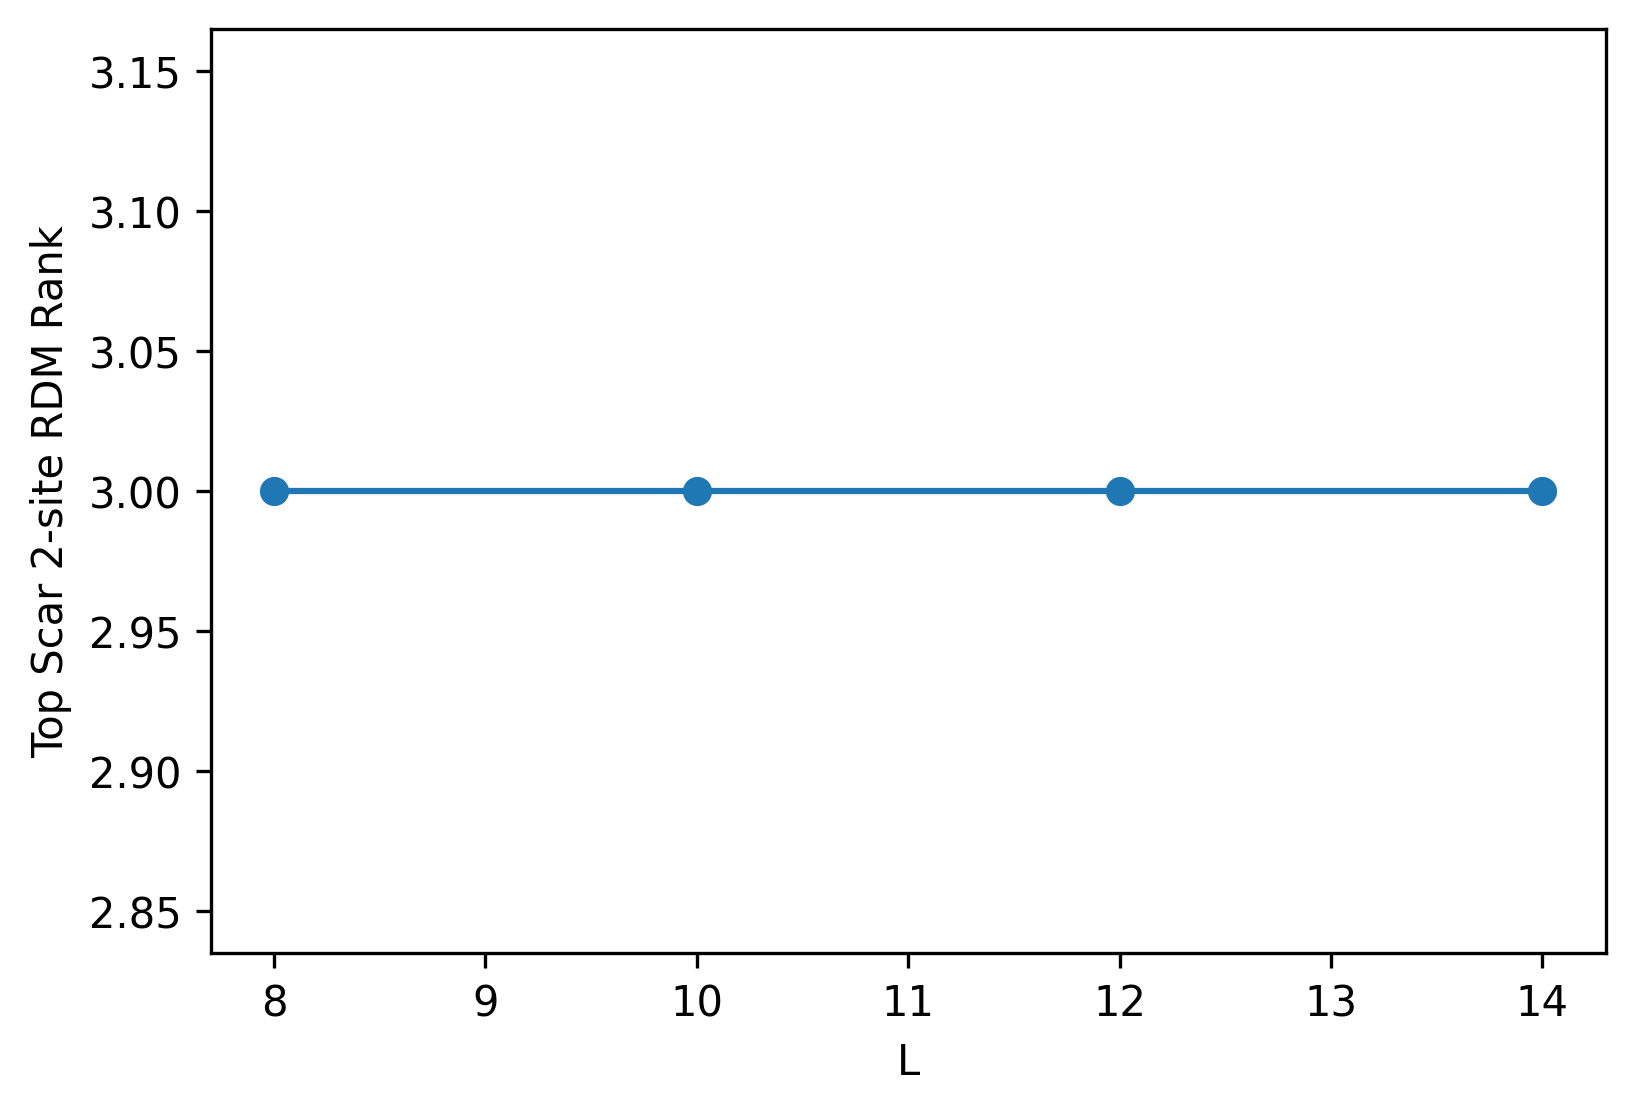
\includegraphics[width=\linewidth]{hb_scar_2.png}
        \caption{}
        \label{fig:image1h}
    \end{subfigure}
    % Second image
    \begin{subfigure}{0.45\textwidth}
        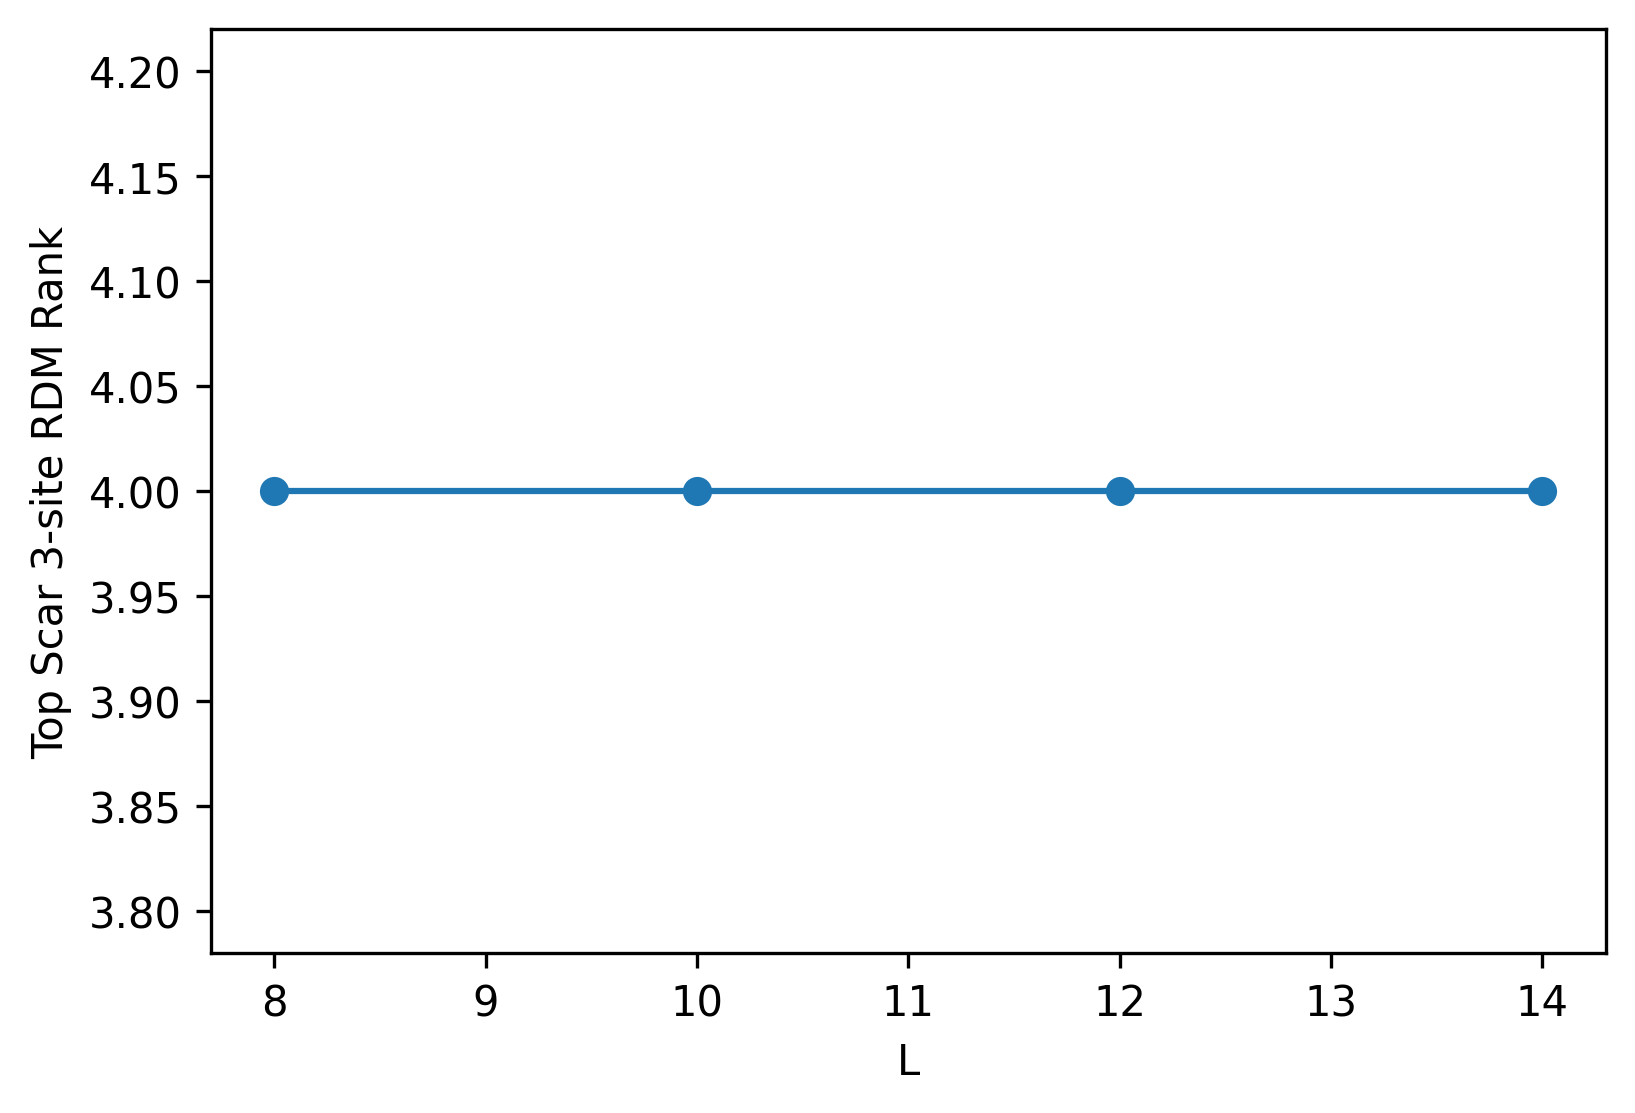
\includegraphics[width=\linewidth]{hb_scar_3.png}
        \caption{}
        \label{fig:image2hb}
    \end{subfigure}    % Third image
    \begin{subfigure}{0.45\textwidth}
        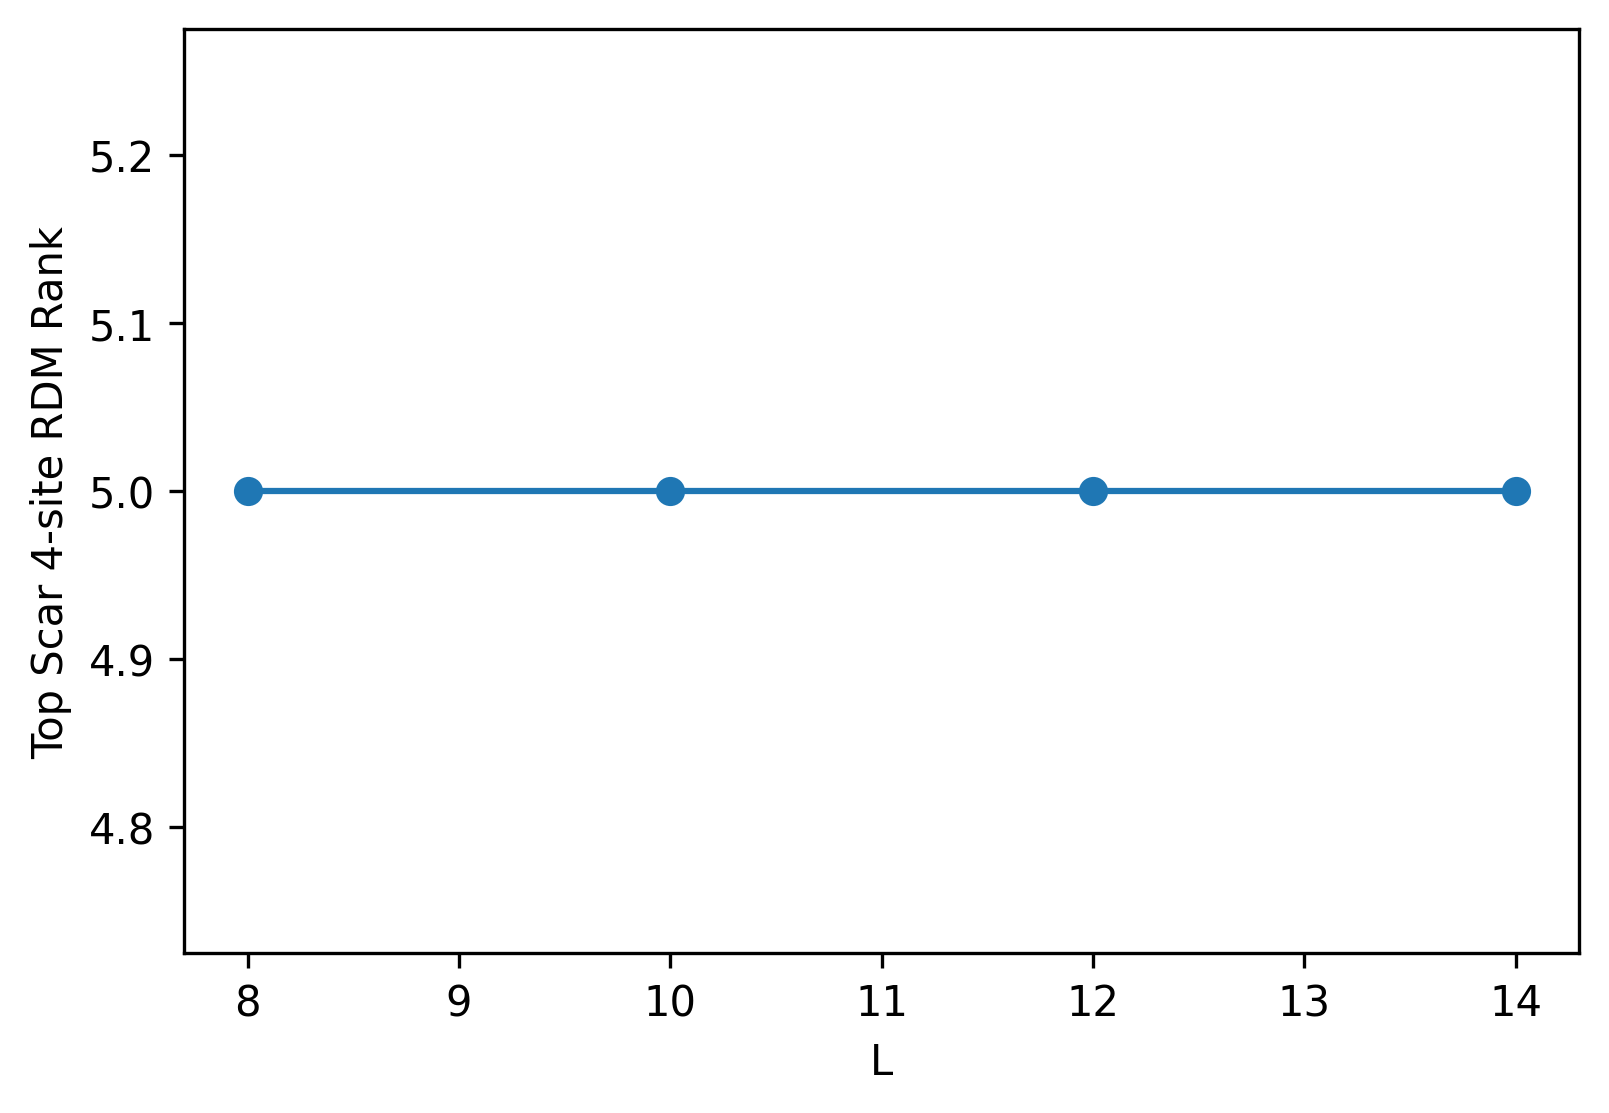
\includegraphics[width=\linewidth]{hb_scar_4.png}
        \caption{}
        \label{fig:image3hb}
    \end{subfigure}

    % Common caption
    \caption{Innermost 2,3,4-sites RDM  rank (Fig. (a), (b), (c) respectively) of the top scar of the tower $|S_n\rangle$ as a function of increasing $L$.}
    \label{fig:hb_scars_tower}
\end{figure}


\end{itemize}


\vspace{0.5cm}
\pagebreak
\section*{Conclusion}

Across all models, the focus was placed exclusively on scarred states with known exact analytic expressions. The investigations confirm key entanglement features and low-rank structure of adjacent reduced density matrices, serving as diagnostics of scarred nonthermal behavior without requiring access to the full spectrum.

\end{document}
